% Options for packages loaded elsewhere
\PassOptionsToPackage{unicode}{hyperref}
\PassOptionsToPackage{hyphens}{url}
%
\documentclass[
  12pt,
]{article}
\usepackage{amsmath,amssymb}
\usepackage{lmodern}
\usepackage{iftex}
\ifPDFTeX
  \usepackage[T1]{fontenc}
  \usepackage[utf8]{inputenc}
  \usepackage{textcomp} % provide euro and other symbols
\else % if luatex or xetex
  \usepackage{unicode-math}
  \defaultfontfeatures{Scale=MatchLowercase}
  \defaultfontfeatures[\rmfamily]{Ligatures=TeX,Scale=1}
  \setmainfont[]{Times New Roman}
\fi
% Use upquote if available, for straight quotes in verbatim environments
\IfFileExists{upquote.sty}{\usepackage{upquote}}{}
\IfFileExists{microtype.sty}{% use microtype if available
  \usepackage[]{microtype}
  \UseMicrotypeSet[protrusion]{basicmath} % disable protrusion for tt fonts
}{}
\makeatletter
\@ifundefined{KOMAClassName}{% if non-KOMA class
  \IfFileExists{parskip.sty}{%
    \usepackage{parskip}
  }{% else
    \setlength{\parindent}{0pt}
    \setlength{\parskip}{6pt plus 2pt minus 1pt}}
}{% if KOMA class
  \KOMAoptions{parskip=half}}
\makeatother
\usepackage{xcolor}
\IfFileExists{xurl.sty}{\usepackage{xurl}}{} % add URL line breaks if available
\IfFileExists{bookmark.sty}{\usepackage{bookmark}}{\usepackage{hyperref}}
\hypersetup{
  pdftitle={Insert title of project here},
  pdfauthor={Name},
  hidelinks,
  pdfcreator={LaTeX via pandoc}}
\urlstyle{same} % disable monospaced font for URLs
\usepackage[margin=2.54cm]{geometry}
\usepackage{color}
\usepackage{fancyvrb}
\newcommand{\VerbBar}{|}
\newcommand{\VERB}{\Verb[commandchars=\\\{\}]}
\DefineVerbatimEnvironment{Highlighting}{Verbatim}{commandchars=\\\{\}}
% Add ',fontsize=\small' for more characters per line
\usepackage{framed}
\definecolor{shadecolor}{RGB}{248,248,248}
\newenvironment{Shaded}{\begin{snugshade}}{\end{snugshade}}
\newcommand{\AlertTok}[1]{\textcolor[rgb]{0.94,0.16,0.16}{#1}}
\newcommand{\AnnotationTok}[1]{\textcolor[rgb]{0.56,0.35,0.01}{\textbf{\textit{#1}}}}
\newcommand{\AttributeTok}[1]{\textcolor[rgb]{0.77,0.63,0.00}{#1}}
\newcommand{\BaseNTok}[1]{\textcolor[rgb]{0.00,0.00,0.81}{#1}}
\newcommand{\BuiltInTok}[1]{#1}
\newcommand{\CharTok}[1]{\textcolor[rgb]{0.31,0.60,0.02}{#1}}
\newcommand{\CommentTok}[1]{\textcolor[rgb]{0.56,0.35,0.01}{\textit{#1}}}
\newcommand{\CommentVarTok}[1]{\textcolor[rgb]{0.56,0.35,0.01}{\textbf{\textit{#1}}}}
\newcommand{\ConstantTok}[1]{\textcolor[rgb]{0.00,0.00,0.00}{#1}}
\newcommand{\ControlFlowTok}[1]{\textcolor[rgb]{0.13,0.29,0.53}{\textbf{#1}}}
\newcommand{\DataTypeTok}[1]{\textcolor[rgb]{0.13,0.29,0.53}{#1}}
\newcommand{\DecValTok}[1]{\textcolor[rgb]{0.00,0.00,0.81}{#1}}
\newcommand{\DocumentationTok}[1]{\textcolor[rgb]{0.56,0.35,0.01}{\textbf{\textit{#1}}}}
\newcommand{\ErrorTok}[1]{\textcolor[rgb]{0.64,0.00,0.00}{\textbf{#1}}}
\newcommand{\ExtensionTok}[1]{#1}
\newcommand{\FloatTok}[1]{\textcolor[rgb]{0.00,0.00,0.81}{#1}}
\newcommand{\FunctionTok}[1]{\textcolor[rgb]{0.00,0.00,0.00}{#1}}
\newcommand{\ImportTok}[1]{#1}
\newcommand{\InformationTok}[1]{\textcolor[rgb]{0.56,0.35,0.01}{\textbf{\textit{#1}}}}
\newcommand{\KeywordTok}[1]{\textcolor[rgb]{0.13,0.29,0.53}{\textbf{#1}}}
\newcommand{\NormalTok}[1]{#1}
\newcommand{\OperatorTok}[1]{\textcolor[rgb]{0.81,0.36,0.00}{\textbf{#1}}}
\newcommand{\OtherTok}[1]{\textcolor[rgb]{0.56,0.35,0.01}{#1}}
\newcommand{\PreprocessorTok}[1]{\textcolor[rgb]{0.56,0.35,0.01}{\textit{#1}}}
\newcommand{\RegionMarkerTok}[1]{#1}
\newcommand{\SpecialCharTok}[1]{\textcolor[rgb]{0.00,0.00,0.00}{#1}}
\newcommand{\SpecialStringTok}[1]{\textcolor[rgb]{0.31,0.60,0.02}{#1}}
\newcommand{\StringTok}[1]{\textcolor[rgb]{0.31,0.60,0.02}{#1}}
\newcommand{\VariableTok}[1]{\textcolor[rgb]{0.00,0.00,0.00}{#1}}
\newcommand{\VerbatimStringTok}[1]{\textcolor[rgb]{0.31,0.60,0.02}{#1}}
\newcommand{\WarningTok}[1]{\textcolor[rgb]{0.56,0.35,0.01}{\textbf{\textit{#1}}}}
\usepackage{graphicx}
\makeatletter
\def\maxwidth{\ifdim\Gin@nat@width>\linewidth\linewidth\else\Gin@nat@width\fi}
\def\maxheight{\ifdim\Gin@nat@height>\textheight\textheight\else\Gin@nat@height\fi}
\makeatother
% Scale images if necessary, so that they will not overflow the page
% margins by default, and it is still possible to overwrite the defaults
% using explicit options in \includegraphics[width, height, ...]{}
\setkeys{Gin}{width=\maxwidth,height=\maxheight,keepaspectratio}
% Set default figure placement to htbp
\makeatletter
\def\fps@figure{htbp}
\makeatother
\setlength{\emergencystretch}{3em} % prevent overfull lines
\providecommand{\tightlist}{%
  \setlength{\itemsep}{0pt}\setlength{\parskip}{0pt}}
\setcounter{secnumdepth}{5}
\ifLuaTeX
  \usepackage{selnolig}  % disable illegal ligatures
\fi

\title{Insert title of project here}
\usepackage{etoolbox}
\makeatletter
\providecommand{\subtitle}[1]{% add subtitle to \maketitle
  \apptocmd{\@title}{\par {\large #1 \par}}{}{}
}
\makeatother
\subtitle{Web address for GitHub repository}
\author{Name}
\date{}

\begin{document}
\maketitle

\newpage
\tableofcontents

Rationale and Research Questions Dataset Information Exploratory
Analysis Analysis Summary and Conclusions References

\newpage
\listoftables

\newpage
\listoffigures

\newpage

\hypertarget{rationale-and-research-questions}{%
\section{Rationale and Research
Questions}\label{rationale-and-research-questions}}

Water is an essential substance for human survival and development. As
the world population increases, living standards improve, water trading
patterns change, and industry, agriculture, and manufacturing expand,
human society's demand for water resources is further expanded (Ercin et
al., 2014). During the last few decades, the scarcity of fresh water is
evidently becoming a threat to the sustainable development of human
societies due to the steady increase in demand. In addition to these
pressures from humans, climate change, including global warming,
significant decreases in precipitation in some areas, and increasingly
frequent extreme weather events, may reduce water production. These
conflicting trends raise further concerns about future water scarcity
(Brown et al., 2013). The 2018 edition of the United Nations (UN) World
Water Development Report (WWDR) presented concerns about water security
that ``the capacity of a population to safeguard sustainable access to
adequate quantities of water with acceptable quality, is already at
risk, and the situation will become worse in the next few decades.'' On
the global scale, there is enough fresh water on an annual basis to meet
the current needs of human society for survival and development
(Vörösmarty, et al., 2000). However, there are great variations of water
availability and water demands on space and time. that is, the
distributions of water resources, population, agriculture, and industry
are uneven, leading to existing water scarcity in several specific parts
of the world during specific times of the year (Mekonnen et al., 2016).
Therefore, the study of long-term water resources capacity for local
areas is significant. The water resources consumed by human society are
generally blue water (fresh surface water and groundwater) (Wada et al.,
2011). Groundwater supplies drinking water for billions of people and
provides nearly half of the water used for agricultural irrigation
(Siebert et al., 2010). It has a perennial distribution suitable for
providing reliable drinking water and supporting efforts to adapt to
extreme natural weather disasters and climate change (Taylor et al.,
2013). In other words, the amount of groundwater is more stable in the
long term compared to the amount of surface water. Surface water,
because of its exposure to the surface, is susceptible to the influence
of external substances. Its water volume also fluctuates greatly under
natural conditions due to temperature, evaporation, sand content and
other factors. And in recent years, influenced by the development of
human activities, the aquifers' shrinkage and salt intrusion in coastal
areas have been increasing dramatically. (Boretti et al., 2019). In this
study, we focus on the Durham region in North Carolina, and hope to
analyze the impact of regional water withdrawal and precipitation on
regional water capacity, including surface water and groundwater,
through data since complete records are available. \#We perform analysis
based on the following sub-questions. \#How is groundwater table related
to precipitation? \#How is groundwater table level related to local
river discharge? \#How is ground water table level related to local
withdraws?

\newpage

\hypertarget{dataset-information}{%
\section{Dataset Information}\label{dataset-information}}

In order to better determine trends and the stability of the water
resource capacity in Durham, it is important to identify the factors
that affect water capacity. We are concerned in this study with the
influence of natural factors and human activities, which are
precipitation and water withdrawal. Data of precipitation in North
Carolina published by National Oceanic and Atmospheric Administration
(NOAA) and water resources depletion value related to human activities
published by the North Carolina Department of Environmental Quality
(NCDEQ) Division of Water Resources are used as the focused factors.
Researching and predicting water depletion requires models of certain
scale, and these models inevitably rely on a variety of simplifying
assumptions. One assumption is that there are no feedbacks between water
supply and water demand. Another assumption is that the flow is
proportional to the river capacity if both the river width and the
riverbed depth remain stable, in another word, the cross-sectional area
of individual parts of the river remains constant. According to the
Local Water Supply Planning published annually by the North Carolina
Department of Environmental Quality (NCDEQ) Division of Water Resources,
the surface water sources of Durham area are mainly Cape Fear Lake, Flat
River and Little River, with the Eno River used as a backup source in
case of emergency. Among these rivers, Flat River, Little River and Eno
River belong to the Neuse River basin, while Cape Fear Lake belongs to
the Haw River basin. United States Geological Survey (USGS) provides
complete flow data for these rivers. While total discharge and
withdrawals are analyzed, we also look for differences in discharge
variability and vulnerability to human activities among the rivers. The
Local Water Supply Planning also describes the destination of treated
sewage in Durham region. According to the report, the treated effluent
flows into Ellerbee River and New Hope River, which belong to Neuse
River basin and Haw River basin respectively. The design receiving
capacity of both rivers is the same, 20 million gallon per day (MGD);
the actual receiving capacity is also approximately the same, about 10
MGD, so it can be assumed that the treated effluent is equally
distributed to the two rivers. From the report, it is clear that the
water withdrawal and discharge points are located in different rivers,
even if they are in the same watershed. Therefore, when considering the
sources of river recharge, we only considered precipitation recharge
without considering the volume of treated wastewater in Durham region.

\newpage

\hypertarget{exploratory-analysis}{%
\section{Exploratory Analysis}\label{exploratory-analysis}}

\begin{Shaded}
\begin{Highlighting}[]
\CommentTok{\#Regular Water Resources}
\NormalTok{CapeFearRiverDischarge }\OtherTok{\textless{}{-}} \FunctionTok{readNWISdv}\NormalTok{(}\AttributeTok{siteNumbers =} \StringTok{"02096500"}\NormalTok{,}
                                  \AttributeTok{parameterCd =} \StringTok{"00060"}\NormalTok{, }\CommentTok{\# discharge (ft3/s)}
                                  \AttributeTok{startDate =} \StringTok{"1990{-}01{-}01"}\NormalTok{,}
                                  \AttributeTok{endDate =} \StringTok{"2021{-}12{-}31"}\NormalTok{)}
\FunctionTok{names}\NormalTok{(CapeFearRiverDischarge)[}\DecValTok{4}\SpecialCharTok{:}\DecValTok{5}\NormalTok{] }\OtherTok{\textless{}{-}} \FunctionTok{c}\NormalTok{(}\StringTok{"CapeFear\_Discharge"}\NormalTok{, }\StringTok{"Approval.Code"}\NormalTok{)}
\FunctionTok{c}\NormalTok{(}\FunctionTok{min}\NormalTok{(CapeFearRiverDischarge}\SpecialCharTok{$}\NormalTok{Date), }\FunctionTok{max}\NormalTok{(CapeFearRiverDischarge}\SpecialCharTok{$}\NormalTok{Date))}
\end{Highlighting}
\end{Shaded}

\begin{verbatim}
## [1] "1990-01-01" "2021-12-31"
\end{verbatim}

\begin{Shaded}
\begin{Highlighting}[]
\CommentTok{\#"1990{-}01{-}01" "2021{-}12{-}31"}
\NormalTok{CapeFearRiverDischarge\_Monthly }\OtherTok{\textless{}{-}}\NormalTok{ CapeFearRiverDischarge }\SpecialCharTok{\%\textgreater{}\%}
  \FunctionTok{mutate}\NormalTok{(}\AttributeTok{Month =} \FunctionTok{format}\NormalTok{(Date,}\StringTok{"\%Y{-}\%m"}\NormalTok{)) }\SpecialCharTok{\%\textgreater{}\%}
  \FunctionTok{group\_by}\NormalTok{(Month) }\SpecialCharTok{\%\textgreater{}\%}
  \FunctionTok{summarise}\NormalTok{(}\AttributeTok{Mean\_CapeFear\_Discharge\_Bymonth =} \FunctionTok{mean}\NormalTok{(CapeFear\_Discharge),}
            \AttributeTok{River =} \FunctionTok{paste}\NormalTok{(}\StringTok{"Cape Fear River"}\NormalTok{))}

\NormalTok{FlatRiverDischarge }\OtherTok{\textless{}{-}} \FunctionTok{readNWISdv}\NormalTok{(}\AttributeTok{siteNumbers =} \StringTok{"02085500"}\NormalTok{,}
                                  \AttributeTok{parameterCd =} \StringTok{"00060"}\NormalTok{, }\CommentTok{\# discharge (ft3/s)}
                                  \AttributeTok{startDate =} \StringTok{"1990{-}01{-}01"}\NormalTok{,}
                                  \AttributeTok{endDate =} \StringTok{"2021{-}12{-}31"}\NormalTok{)}
\FunctionTok{names}\NormalTok{(FlatRiverDischarge)[}\DecValTok{4}\SpecialCharTok{:}\DecValTok{5}\NormalTok{] }\OtherTok{\textless{}{-}} \FunctionTok{c}\NormalTok{(}\StringTok{"Flat\_Discharge"}\NormalTok{, }\StringTok{"Approval.Code"}\NormalTok{)}
\FunctionTok{c}\NormalTok{(}\FunctionTok{min}\NormalTok{(FlatRiverDischarge}\SpecialCharTok{$}\NormalTok{Date), }\FunctionTok{max}\NormalTok{(FlatRiverDischarge}\SpecialCharTok{$}\NormalTok{Date))}
\end{Highlighting}
\end{Shaded}

\begin{verbatim}
## [1] "1990-01-01" "2021-12-31"
\end{verbatim}

\begin{Shaded}
\begin{Highlighting}[]
\CommentTok{\#"1990{-}01{-}01" "2021{-}12{-}31"}
\NormalTok{FlatRiverDischarge\_Monthly }\OtherTok{\textless{}{-}}\NormalTok{ FlatRiverDischarge }\SpecialCharTok{\%\textgreater{}\%}
  \FunctionTok{mutate}\NormalTok{(}\AttributeTok{Month =} \FunctionTok{format}\NormalTok{(Date,}\StringTok{"\%Y{-}\%m"}\NormalTok{)) }\SpecialCharTok{\%\textgreater{}\%}
  \FunctionTok{group\_by}\NormalTok{(Month) }\SpecialCharTok{\%\textgreater{}\%}
  \FunctionTok{summarise}\NormalTok{(}\AttributeTok{Mean\_Flat\_Discharge\_Bymonth =} \FunctionTok{mean}\NormalTok{(Flat\_Discharge),}
            \AttributeTok{River =} \FunctionTok{paste}\NormalTok{(}\StringTok{"Flat River"}\NormalTok{))}

\NormalTok{LittleRiverDischarge }\OtherTok{\textless{}{-}} \FunctionTok{readNWISdv}\NormalTok{(}\AttributeTok{siteNumbers =} \StringTok{"0208524975"}\NormalTok{,}
                                  \AttributeTok{parameterCd =} \StringTok{"00060"}\NormalTok{, }\CommentTok{\# discharge (ft3/s)}
                                  \AttributeTok{startDate =} \StringTok{"1990{-}01{-}01"}\NormalTok{,}
                                  \AttributeTok{endDate =} \StringTok{"2021{-}12{-}31"}\NormalTok{)}
\FunctionTok{names}\NormalTok{(LittleRiverDischarge)[}\DecValTok{4}\SpecialCharTok{:}\DecValTok{5}\NormalTok{] }\OtherTok{\textless{}{-}} \FunctionTok{c}\NormalTok{(}\StringTok{"Little\_Discharge"}\NormalTok{, }\StringTok{"Approval.Code"}\NormalTok{)}
\FunctionTok{c}\NormalTok{(}\FunctionTok{min}\NormalTok{(LittleRiverDischarge}\SpecialCharTok{$}\NormalTok{Date), }\FunctionTok{max}\NormalTok{(LittleRiverDischarge}\SpecialCharTok{$}\NormalTok{Date))}
\end{Highlighting}
\end{Shaded}

\begin{verbatim}
## [1] "1995-10-24" "2021-12-31"
\end{verbatim}

\begin{Shaded}
\begin{Highlighting}[]
\CommentTok{\#"1995{-}10{-}24" "2021{-}12{-}31"}
\NormalTok{LittleRiverDischarge\_Monthly }\OtherTok{\textless{}{-}}\NormalTok{ LittleRiverDischarge }\SpecialCharTok{\%\textgreater{}\%}
  \FunctionTok{mutate}\NormalTok{(}\AttributeTok{Month =} \FunctionTok{format}\NormalTok{(Date,}\StringTok{"\%Y{-}\%m"}\NormalTok{)) }\SpecialCharTok{\%\textgreater{}\%}
  \FunctionTok{group\_by}\NormalTok{(Month) }\SpecialCharTok{\%\textgreater{}\%}
  \FunctionTok{summarise}\NormalTok{(}\AttributeTok{Mean\_Little\_Discharge\_Bymonth =} \FunctionTok{mean}\NormalTok{(Little\_Discharge),}
            \AttributeTok{River =} \FunctionTok{paste}\NormalTok{(}\StringTok{"Little River"}\NormalTok{))}

\CommentTok{\#Emergency Water Resources}
\NormalTok{EnoRiverDischarge }\OtherTok{\textless{}{-}} \FunctionTok{readNWISdv}\NormalTok{(}\AttributeTok{siteNumbers =} \StringTok{"02085070"}\NormalTok{,}
                                  \AttributeTok{parameterCd =} \StringTok{"00060"}\NormalTok{, }\CommentTok{\# discharge (ft3/s)}
                                  \AttributeTok{startDate =} \StringTok{"1990{-}01{-}01"}\NormalTok{,}
                                  \AttributeTok{endDate =} \StringTok{"2021{-}12{-}31"}\NormalTok{)}
\FunctionTok{names}\NormalTok{(EnoRiverDischarge)[}\DecValTok{4}\SpecialCharTok{:}\DecValTok{5}\NormalTok{] }\OtherTok{\textless{}{-}} \FunctionTok{c}\NormalTok{(}\StringTok{"Discharge"}\NormalTok{, }\StringTok{"Approval.Code"}\NormalTok{)}
\FunctionTok{c}\NormalTok{(}\FunctionTok{min}\NormalTok{(EnoRiverDischarge}\SpecialCharTok{$}\NormalTok{Date), }\FunctionTok{max}\NormalTok{(EnoRiverDischarge}\SpecialCharTok{$}\NormalTok{Date))}
\end{Highlighting}
\end{Shaded}

\begin{verbatim}
## [1] "1990-01-01" "2021-12-31"
\end{verbatim}

\begin{Shaded}
\begin{Highlighting}[]
\CommentTok{\#"1990{-}01{-}01" "2021{-}12{-}31"}
\NormalTok{EnoRiverDischarge\_Monthly }\OtherTok{\textless{}{-}}\NormalTok{ EnoRiverDischarge }\SpecialCharTok{\%\textgreater{}\%}
  \FunctionTok{mutate}\NormalTok{(}\AttributeTok{Month =} \FunctionTok{format}\NormalTok{(Date,}\StringTok{"\%Y{-}\%m"}\NormalTok{)) }\SpecialCharTok{\%\textgreater{}\%}
  \FunctionTok{group\_by}\NormalTok{(Month) }\SpecialCharTok{\%\textgreater{}\%}
  \FunctionTok{summarise}\NormalTok{(}\AttributeTok{Mean\_Discharge\_Bymonth =} \FunctionTok{mean}\NormalTok{(Discharge),}
            \AttributeTok{River =} \FunctionTok{paste}\NormalTok{(}\StringTok{"Eno River"}\NormalTok{))}

\CommentTok{\#Surrounding Water Resources (Unused)}
\NormalTok{EllerbeCreekDischarge }\OtherTok{\textless{}{-}} \FunctionTok{readNWISdv}\NormalTok{(}\AttributeTok{siteNumbers =} \StringTok{"0208675010"}\NormalTok{,}
                                  \AttributeTok{parameterCd =} \StringTok{"00060"}\NormalTok{, }\CommentTok{\# discharge (ft3/s)}
                                  \AttributeTok{startDate =} \StringTok{"1990{-}01{-}01"}\NormalTok{,}
                                  \AttributeTok{endDate =} \StringTok{"2021{-}12{-}31"}\NormalTok{)}
\FunctionTok{names}\NormalTok{(EllerbeCreekDischarge)[}\DecValTok{4}\SpecialCharTok{:}\DecValTok{5}\NormalTok{] }\OtherTok{\textless{}{-}} \FunctionTok{c}\NormalTok{(}\StringTok{"Discharge"}\NormalTok{, }\StringTok{"Approval.Code"}\NormalTok{)}
\FunctionTok{c}\NormalTok{(}\FunctionTok{min}\NormalTok{(EllerbeCreekDischarge}\SpecialCharTok{$}\NormalTok{Date), }\FunctionTok{max}\NormalTok{(EllerbeCreekDischarge}\SpecialCharTok{$}\NormalTok{Date))}
\end{Highlighting}
\end{Shaded}

\begin{verbatim}
## [1] "2008-08-01" "2021-12-31"
\end{verbatim}

\begin{Shaded}
\begin{Highlighting}[]
\CommentTok{\#"2008{-}08{-}01" "2021{-}12{-}31"}
\NormalTok{EllerbeCreekDischarge\_Monthly }\OtherTok{\textless{}{-}}\NormalTok{ EllerbeCreekDischarge }\SpecialCharTok{\%\textgreater{}\%}
  \FunctionTok{mutate}\NormalTok{(}\AttributeTok{Month =} \FunctionTok{format}\NormalTok{(Date,}\StringTok{"\%Y{-}\%m"}\NormalTok{)) }\SpecialCharTok{\%\textgreater{}\%}
  \FunctionTok{group\_by}\NormalTok{(Month) }\SpecialCharTok{\%\textgreater{}\%}
  \FunctionTok{summarise}\NormalTok{(}\AttributeTok{Mean\_Discharge\_Bymonth =} \FunctionTok{mean}\NormalTok{(Discharge),}
            \AttributeTok{River =} \FunctionTok{paste}\NormalTok{(}\StringTok{"Ellerbe Creek"}\NormalTok{))}

\NormalTok{SandyCreekDischarge }\OtherTok{\textless{}{-}} \FunctionTok{readNWISdv}\NormalTok{(}\AttributeTok{siteNumbers =} \StringTok{"0209722970"}\NormalTok{,}
                                  \AttributeTok{parameterCd =} \StringTok{"00060"}\NormalTok{, }\CommentTok{\# discharge (ft3/s)}
                                  \AttributeTok{startDate =} \StringTok{"1990{-}01{-}01"}\NormalTok{,}
                                  \AttributeTok{endDate =} \StringTok{"2021{-}12{-}31"}\NormalTok{)}
\FunctionTok{names}\NormalTok{(SandyCreekDischarge)[}\DecValTok{4}\SpecialCharTok{:}\DecValTok{5}\NormalTok{] }\OtherTok{\textless{}{-}} \FunctionTok{c}\NormalTok{(}\StringTok{"Discharge"}\NormalTok{, }\StringTok{"Approval.Code"}\NormalTok{)}
\FunctionTok{c}\NormalTok{(}\FunctionTok{min}\NormalTok{(SandyCreekDischarge}\SpecialCharTok{$}\NormalTok{Date), }\FunctionTok{max}\NormalTok{(SandyCreekDischarge}\SpecialCharTok{$}\NormalTok{Date))}
\end{Highlighting}
\end{Shaded}

\begin{verbatim}
## [1] "2008-08-01" "2021-12-31"
\end{verbatim}

\begin{Shaded}
\begin{Highlighting}[]
\CommentTok{\#"2008{-}08{-}01" "2021{-}12{-}31"}
\NormalTok{SandyCreekDischarge\_Monthly }\OtherTok{\textless{}{-}}\NormalTok{ SandyCreekDischarge }\SpecialCharTok{\%\textgreater{}\%}
  \FunctionTok{mutate}\NormalTok{(}\AttributeTok{Month =} \FunctionTok{format}\NormalTok{(Date,}\StringTok{"\%Y{-}\%m"}\NormalTok{)) }\SpecialCharTok{\%\textgreater{}\%}
  \FunctionTok{group\_by}\NormalTok{(Month) }\SpecialCharTok{\%\textgreater{}\%}
  \FunctionTok{summarise}\NormalTok{(}\AttributeTok{Mean\_Discharge\_Bymonth =} \FunctionTok{mean}\NormalTok{(Discharge),}
            \AttributeTok{River =} \FunctionTok{paste}\NormalTok{(}\StringTok{"Sandy Creek"}\NormalTok{))}

\NormalTok{ThirdForkCreekDischarge }\OtherTok{\textless{}{-}} \FunctionTok{readNWISdv}\NormalTok{(}\AttributeTok{siteNumbers =} \StringTok{"0209725960"}\NormalTok{,}
                                  \AttributeTok{parameterCd =} \StringTok{"00060"}\NormalTok{, }\CommentTok{\# discharge (ft3/s)}
                                  \AttributeTok{startDate =} \StringTok{"1990{-}01{-}01"}\NormalTok{,}
                                  \AttributeTok{endDate =} \StringTok{"2021{-}12{-}31"}\NormalTok{)}
\FunctionTok{names}\NormalTok{(ThirdForkCreekDischarge)[}\DecValTok{4}\SpecialCharTok{:}\DecValTok{5}\NormalTok{] }\OtherTok{\textless{}{-}} \FunctionTok{c}\NormalTok{(}\StringTok{"Discharge"}\NormalTok{, }\StringTok{"Approval.Code"}\NormalTok{)}
\FunctionTok{c}\NormalTok{(}\FunctionTok{min}\NormalTok{(ThirdForkCreekDischarge}\SpecialCharTok{$}\NormalTok{Date), }\FunctionTok{max}\NormalTok{(ThirdForkCreekDischarge}\SpecialCharTok{$}\NormalTok{Date))}
\end{Highlighting}
\end{Shaded}

\begin{verbatim}
## [1] "2017-06-16" "2021-12-31"
\end{verbatim}

\begin{Shaded}
\begin{Highlighting}[]
\CommentTok{\#"2017{-}06{-}16" "2021{-}12{-}31"}
\NormalTok{ThirdForkCreekDischarge\_Monthly }\OtherTok{\textless{}{-}}\NormalTok{ ThirdForkCreekDischarge }\SpecialCharTok{\%\textgreater{}\%}
  \FunctionTok{mutate}\NormalTok{(}\AttributeTok{Month =} \FunctionTok{format}\NormalTok{(Date,}\StringTok{"\%Y{-}\%m"}\NormalTok{)) }\SpecialCharTok{\%\textgreater{}\%}
  \FunctionTok{group\_by}\NormalTok{(Month) }\SpecialCharTok{\%\textgreater{}\%}
  \FunctionTok{summarise}\NormalTok{(}\AttributeTok{Mean\_Discharge\_Bymonth =} \FunctionTok{mean}\NormalTok{(Discharge),}
            \AttributeTok{River =} \FunctionTok{paste}\NormalTok{(}\StringTok{"Third Fork Creek"}\NormalTok{))}
\end{Highlighting}
\end{Shaded}

\begin{Shaded}
\begin{Highlighting}[]
\NormalTok{GroundParams }\OtherTok{\textless{}{-}} \FunctionTok{whatNWISdata}\NormalTok{(}\AttributeTok{siteNumbers =} \StringTok{"355944079013401"}\NormalTok{)}
\NormalTok{DurhamGroundwater }\OtherTok{\textless{}{-}} \FunctionTok{readNWISdv}\NormalTok{(}\AttributeTok{siteNumbers =} \StringTok{"355944079013401"}\NormalTok{, }\CommentTok{\#Duke Forest}
                                 \AttributeTok{parameterCd =} \StringTok{"72019"}\NormalTok{, }\CommentTok{\# /62610/Groundwater level above NGVD 1929 (feet)}
                                 \AttributeTok{statCd =} \StringTok{"00002"}\NormalTok{,}
                                 \AttributeTok{startDate =} \StringTok{"2014{-}01{-}01"}\NormalTok{,}
                                 \AttributeTok{endDate =} \StringTok{"2021{-}12{-}31"}\NormalTok{)}
\FunctionTok{colnames}\NormalTok{(DurhamGroundwater) }\OtherTok{\textless{}{-}} \FunctionTok{c}\NormalTok{(}\StringTok{"Agency\_Name"}\NormalTok{,}
                                 \StringTok{"Site\_Number"}\NormalTok{,}
                                 \StringTok{"Date"}\NormalTok{,}
                                 \StringTok{"Groundwater\_Table\_feet"}\NormalTok{, }
                                 \StringTok{"Approval.Code"}\NormalTok{)}
\FunctionTok{summary}\NormalTok{(DurhamGroundwater)}
\end{Highlighting}
\end{Shaded}

\begin{verbatim}
##  Agency_Name        Site_Number             Date           
##  Length:2911        Length:2911        Min.   :2014-01-01  
##  Class :character   Class :character   1st Qu.:2015-12-29  
##  Mode  :character   Mode  :character   Median :2017-12-27  
##                                        Mean   :2017-12-29  
##                                        3rd Qu.:2019-12-27  
##                                        Max.   :2021-12-31  
##  Groundwater_Table_feet Approval.Code     
##  Min.   :34.12          Length:2911       
##  1st Qu.:37.28          Class :character  
##  Median :39.15          Mode  :character  
##  Mean   :38.76                            
##  3rd Qu.:40.34                            
##  Max.   :42.22
\end{verbatim}

\begin{Shaded}
\begin{Highlighting}[]
\FunctionTok{head}\NormalTok{(DurhamGroundwater)}
\end{Highlighting}
\end{Shaded}

\begin{verbatim}
##   Agency_Name     Site_Number       Date Groundwater_Table_feet Approval.Code
## 1        USGS 355944079013401 2014-01-01                  42.18             A
## 2        USGS 355944079013401 2014-01-02                  42.07             A
## 3        USGS 355944079013401 2014-01-03                  42.15             A
## 4        USGS 355944079013401 2014-01-04                  42.17             A
## 5        USGS 355944079013401 2014-01-05                  42.08             A
## 6        USGS 355944079013401 2014-01-06                  42.05             A
\end{verbatim}

\begin{Shaded}
\begin{Highlighting}[]
\NormalTok{DurhamGroundwater\_Monthly }\OtherTok{\textless{}{-}}\NormalTok{ DurhamGroundwater }\SpecialCharTok{\%\textgreater{}\%}
  \FunctionTok{mutate}\NormalTok{(}\AttributeTok{Month =} \FunctionTok{format}\NormalTok{(Date,}\StringTok{"\%Y{-}\%m"}\NormalTok{)) }\SpecialCharTok{\%\textgreater{}\%}
  \FunctionTok{group\_by}\NormalTok{(Month) }\SpecialCharTok{\%\textgreater{}\%}
  \FunctionTok{summarise}\NormalTok{(}\AttributeTok{Mean\_Groundwater\_Table\_feet =} \FunctionTok{mean}\NormalTok{(Groundwater\_Table\_feet))}
\end{Highlighting}
\end{Shaded}

\begin{Shaded}
\begin{Highlighting}[]
\CommentTok{\#the PSWID of Durham}
\NormalTok{durham\_pswid }\OtherTok{=} \StringTok{\textquotesingle{}03{-}32{-}010\textquotesingle{}}
\CommentTok{\#years with records}
\NormalTok{the\_years }\OtherTok{=} \FunctionTok{c}\NormalTok{(}\DecValTok{2018}\SpecialCharTok{:}\DecValTok{2021}\NormalTok{)}

\CommentTok{\#Scrap Function}
\NormalTok{scrape.totalwithdrawal }\OtherTok{\textless{}{-}} \ControlFlowTok{function}\NormalTok{(the\_pswid, the\_year)\{}
\NormalTok{  the\_website }\OtherTok{\textless{}{-}} \FunctionTok{read\_html}\NormalTok{(}\FunctionTok{paste0}\NormalTok{(}\StringTok{\textquotesingle{}https://www.ncwater.org/WUDC/app/LWSP/report.php?pwsid=\textquotesingle{}}\NormalTok{, }
\NormalTok{                                  the\_pswid, }\StringTok{\textquotesingle{}\&year=\textquotesingle{}}\NormalTok{, the\_year))}
  
\NormalTok{  water\_system\_name\_tag }\OtherTok{\textless{}{-}} \StringTok{\textquotesingle{}div+ table tr:nth{-}child(1) td:nth{-}child(2)\textquotesingle{}}
\NormalTok{  ownership\_tag }\OtherTok{\textless{}{-}} \StringTok{\textquotesingle{}div+ table tr:nth{-}child(2) td:nth{-}child(4)\textquotesingle{}}
\NormalTok{  avg\_daily\_use\_tag }\OtherTok{\textless{}{-}} \StringTok{\textquotesingle{}.fancy{-}table:nth{-}child(31) th+ td\textquotesingle{}}
  
\NormalTok{  water\_system\_name }\OtherTok{\textless{}{-}}\NormalTok{ the\_website }\SpecialCharTok{\%\textgreater{}\%} \FunctionTok{html\_nodes}\NormalTok{(water\_system\_name\_tag) }\SpecialCharTok{\%\textgreater{}\%} \FunctionTok{html\_text}\NormalTok{()}
\NormalTok{  ownership }\OtherTok{\textless{}{-}}\NormalTok{ the\_website }\SpecialCharTok{\%\textgreater{}\%}   \FunctionTok{html\_nodes}\NormalTok{(ownership\_tag) }\SpecialCharTok{\%\textgreater{}\%}  \FunctionTok{html\_text}\NormalTok{()}
\NormalTok{  avg\_daily\_use }\OtherTok{\textless{}{-}}\NormalTok{ the\_website }\SpecialCharTok{\%\textgreater{}\%} \FunctionTok{html\_nodes}\NormalTok{(avg\_daily\_use\_tag) }\SpecialCharTok{\%\textgreater{}\%} \FunctionTok{html\_text}\NormalTok{()}
  
\NormalTok{  df\_withdrawals }\OtherTok{\textless{}{-}} \FunctionTok{data.frame}\NormalTok{(}\StringTok{"Year"} \OtherTok{=} \FunctionTok{rep}\NormalTok{(the\_year,}\DecValTok{12}\NormalTok{),}
                               \StringTok{"Month"} \OtherTok{=} \FunctionTok{rep}\NormalTok{(}\DecValTok{1}\SpecialCharTok{:}\DecValTok{12}\NormalTok{),}
                               \StringTok{"Avg\_Daily\_Use\_mgd"} \OtherTok{=} \FunctionTok{as.numeric}\NormalTok{(avg\_daily\_use)) }\SpecialCharTok{\%\textgreater{}\%} 
    \FunctionTok{mutate}\NormalTok{(}\AttributeTok{Water\_System\_name =} \SpecialCharTok{!!}\NormalTok{water\_system\_name,}
         \AttributeTok{Ownership =} \SpecialCharTok{!!}\NormalTok{ownership,}
         \AttributeTok{Date =} \FunctionTok{my}\NormalTok{(}\FunctionTok{paste}\NormalTok{(Month,}\StringTok{"{-}"}\NormalTok{,Year)))}
  
  \FunctionTok{print}\NormalTok{(}\FunctionTok{paste}\NormalTok{(}\StringTok{\textquotesingle{}The Pswid =\textquotesingle{}}\NormalTok{, the\_pswid, }\StringTok{\textquotesingle{}, The Year =\textquotesingle{}}\NormalTok{, the\_year))}
  \FunctionTok{return}\NormalTok{(df\_withdrawals)}
\NormalTok{\}}

\NormalTok{total\_withdrawal }\OtherTok{\textless{}{-}} \FunctionTok{map}\NormalTok{(the\_years, scrape.totalwithdrawal, }\AttributeTok{the\_pswid =}\NormalTok{ durham\_pswid)}
\end{Highlighting}
\end{Shaded}

\begin{verbatim}
## [1] "The Pswid = 03-32-010 , The Year = 2018"
## [1] "The Pswid = 03-32-010 , The Year = 2019"
## [1] "The Pswid = 03-32-010 , The Year = 2020"
## [1] "The Pswid = 03-32-010 , The Year = 2021"
\end{verbatim}

\begin{Shaded}
\begin{Highlighting}[]
\NormalTok{total\_withdrawal }\OtherTok{\textless{}{-}} \FunctionTok{bind\_rows}\NormalTok{(total\_withdrawal)}

\NormalTok{total\_withdrawal }\OtherTok{\textless{}{-}} \FunctionTok{read.csv}\NormalTok{(}\StringTok{"../Data/Processed/Durham\_Withdrawal\_Processed.csv"}\NormalTok{)}
\NormalTok{total\_withdrawal}\SpecialCharTok{$}\NormalTok{Date }\OtherTok{\textless{}{-}} \FunctionTok{as\_date}\NormalTok{(total\_withdrawal}\SpecialCharTok{$}\NormalTok{Date, }\AttributeTok{format =} \StringTok{"\%m/\%d/\%y"}\NormalTok{)}

\NormalTok{total\_withdrawal\_Monthly }\OtherTok{\textless{}{-}}\NormalTok{ total\_withdrawal }\SpecialCharTok{\%\textgreater{}\%}
  \FunctionTok{select}\NormalTok{(Date, Avg\_Daily\_Use\_mgd) }\SpecialCharTok{\%\textgreater{}\%}
  \FunctionTok{mutate}\NormalTok{(}\AttributeTok{Month =} \FunctionTok{format}\NormalTok{(Date,}\StringTok{"\%Y{-}\%m"}\NormalTok{)) }\SpecialCharTok{\%\textgreater{}\%}
  \FunctionTok{group\_by}\NormalTok{(Month) }\SpecialCharTok{\%\textgreater{}\%}
  \FunctionTok{summarise}\NormalTok{(}\AttributeTok{Mean\_Avg\_Daily\_Use\_mgd =} \FunctionTok{mean}\NormalTok{(Avg\_Daily\_Use\_mgd))}
\end{Highlighting}
\end{Shaded}

\begin{Shaded}
\begin{Highlighting}[]
\CommentTok{\#the PSWID of Durham}
\NormalTok{durham\_pswid }\OtherTok{=} \StringTok{\textquotesingle{}03{-}32{-}010\textquotesingle{}}
\CommentTok{\#years with records}
\NormalTok{the\_years }\OtherTok{=} \FunctionTok{c}\NormalTok{(}\DecValTok{2018}\SpecialCharTok{:}\DecValTok{2021}\NormalTok{)}

\NormalTok{scrape.withdrawal.distribution }\OtherTok{\textless{}{-}} \ControlFlowTok{function}\NormalTok{(the\_pswid, the\_year)\{}
\NormalTok{  the\_website }\OtherTok{\textless{}{-}} \FunctionTok{read\_html}\NormalTok{(}\FunctionTok{paste0}\NormalTok{(}\StringTok{\textquotesingle{}https://www.ncwater.org/WUDC/app/LWSP/report.php?pwsid=\textquotesingle{}}\NormalTok{, }
\NormalTok{                                  the\_pswid, }\StringTok{\textquotesingle{}\&year=\textquotesingle{}}\NormalTok{, the\_year))}
  
\NormalTok{  water\_system\_name\_tag }\OtherTok{\textless{}{-}} \StringTok{\textquotesingle{}div+ table tr:nth{-}child(1) td:nth{-}child(2)\textquotesingle{}}
\NormalTok{  ownership\_tag }\OtherTok{\textless{}{-}} \StringTok{\textquotesingle{}div+ table tr:nth{-}child(2) td:nth{-}child(4)\textquotesingle{}}
\NormalTok{  stream\_name\_tag }\OtherTok{\textless{}{-}} \StringTok{\textquotesingle{}.fancy{-}table:nth{-}child(35) .left:nth{-}child(1)\textquotesingle{}}
\NormalTok{  avg\_daily\_use\_tag }\OtherTok{\textless{}{-}} \StringTok{\textquotesingle{}.fancy{-}table:nth{-}child(35) .left\textasciitilde{} .left+ td\textquotesingle{}}
\NormalTok{  the\_numberofdaysused\_tag }\OtherTok{\textless{}{-}} \StringTok{\textquotesingle{}.fancy{-}table:nth{-}child(35) td:nth{-}child(4)\textquotesingle{}}
  
\NormalTok{  water\_system\_name }\OtherTok{\textless{}{-}}\NormalTok{ the\_website }\SpecialCharTok{\%\textgreater{}\%} \FunctionTok{html\_nodes}\NormalTok{(water\_system\_name\_tag) }\SpecialCharTok{\%\textgreater{}\%} \FunctionTok{html\_text}\NormalTok{()}
\NormalTok{  ownership }\OtherTok{\textless{}{-}}\NormalTok{ the\_website }\SpecialCharTok{\%\textgreater{}\%}   \FunctionTok{html\_nodes}\NormalTok{(ownership\_tag) }\SpecialCharTok{\%\textgreater{}\%}  \FunctionTok{html\_text}\NormalTok{()}
\NormalTok{  stream\_name }\OtherTok{\textless{}{-}}\NormalTok{ the\_website }\SpecialCharTok{\%\textgreater{}\%} \FunctionTok{html\_nodes}\NormalTok{(stream\_name\_tag) }\SpecialCharTok{\%\textgreater{}\%} \FunctionTok{html\_text}\NormalTok{()}
\NormalTok{  avg\_daily\_use }\OtherTok{\textless{}{-}}\NormalTok{ the\_website }\SpecialCharTok{\%\textgreater{}\%} \FunctionTok{html\_nodes}\NormalTok{(avg\_daily\_use\_tag) }\SpecialCharTok{\%\textgreater{}\%} \FunctionTok{html\_text}\NormalTok{()}
\NormalTok{  the\_numberofdaysused }\OtherTok{\textless{}{-}}\NormalTok{ the\_website }\SpecialCharTok{\%\textgreater{}\%} \FunctionTok{html\_nodes}\NormalTok{(the\_numberofdaysused\_tag) }\SpecialCharTok{\%\textgreater{}\%} \FunctionTok{html\_text}\NormalTok{()}
  
\NormalTok{  df\_withdrawals }\OtherTok{\textless{}{-}} \FunctionTok{data.frame}\NormalTok{(}\StringTok{"Year"} \OtherTok{=} \FunctionTok{rep}\NormalTok{(the\_year,}\DecValTok{5}\NormalTok{),}
                               \StringTok{"Stream\_Name"} \OtherTok{=}\NormalTok{ stream\_name,}
                               \StringTok{"Avg\_Daily\_Use\_mgd"} \OtherTok{=} \FunctionTok{as.numeric}\NormalTok{(avg\_daily\_use),}
                               \StringTok{"Number\_of\_Days\_Used"} \OtherTok{=} \FunctionTok{as.numeric}\NormalTok{(the\_numberofdaysused)) }\SpecialCharTok{\%\textgreater{}\%} 
    \FunctionTok{mutate}\NormalTok{(}\AttributeTok{Water\_System\_name =} \SpecialCharTok{!!}\NormalTok{water\_system\_name,}
         \AttributeTok{Ownership =} \SpecialCharTok{!!}\NormalTok{ownership)}
  
  \FunctionTok{print}\NormalTok{(}\FunctionTok{paste}\NormalTok{(}\StringTok{\textquotesingle{}The Pswid =\textquotesingle{}}\NormalTok{, the\_pswid, }\StringTok{\textquotesingle{}, The Year =\textquotesingle{}}\NormalTok{, the\_year))}
  \FunctionTok{return}\NormalTok{(df\_withdrawals)}
\NormalTok{\}}

\NormalTok{withdrawal\_distribution }\OtherTok{\textless{}{-}} \FunctionTok{map}\NormalTok{(the\_years, scrape.withdrawal.distribution, }\AttributeTok{the\_pswid =}\NormalTok{ durham\_pswid)}
\end{Highlighting}
\end{Shaded}

\begin{verbatim}
## [1] "The Pswid = 03-32-010 , The Year = 2018"
## [1] "The Pswid = 03-32-010 , The Year = 2019"
## [1] "The Pswid = 03-32-010 , The Year = 2020"
## [1] "The Pswid = 03-32-010 , The Year = 2021"
\end{verbatim}

\begin{Shaded}
\begin{Highlighting}[]
\NormalTok{withdrawal\_distribution }\OtherTok{\textless{}{-}} \FunctionTok{bind\_rows}\NormalTok{(withdrawal\_distribution)}
\end{Highlighting}
\end{Shaded}

\begin{Shaded}
\begin{Highlighting}[]
\CommentTok{\#Precipitation}
\NormalTok{PreciParams }\OtherTok{\textless{}{-}} \FunctionTok{whatNWISdata}\NormalTok{(}\AttributeTok{siteNumbers =} \StringTok{"355852078572045"}\NormalTok{)}
\NormalTok{DurhamPrecipitaion }\OtherTok{\textless{}{-}} \FunctionTok{readNWISdv}\NormalTok{(}\AttributeTok{siteNumbers =} \StringTok{"355852078572045"}\NormalTok{,}
                                 \AttributeTok{parameterCd =} \StringTok{"00045"}\NormalTok{, }\CommentTok{\# precipitation (inches)}
                                 \AttributeTok{statCd =} \StringTok{"00006"}\NormalTok{,}
                                 \AttributeTok{startDate =} \StringTok{"2009{-}01{-}01"}\NormalTok{,}
                                 \AttributeTok{endDate =} \StringTok{"2021{-}12{-}31"}\NormalTok{)}
\FunctionTok{colnames}\NormalTok{(DurhamPrecipitaion) }\OtherTok{\textless{}{-}} \FunctionTok{c}\NormalTok{(}\StringTok{"Agency\_Name"}\NormalTok{,}
                                 \StringTok{"Site\_Number"}\NormalTok{,}
                                 \StringTok{"Date"}\NormalTok{,}
                                 \StringTok{"Precipitaion\_inches"}\NormalTok{, }
                                 \StringTok{"Approval.Code"}\NormalTok{)}
\FunctionTok{summary}\NormalTok{(DurhamPrecipitaion)}
\end{Highlighting}
\end{Shaded}

\begin{verbatim}
##  Agency_Name        Site_Number             Date            Precipitaion_inches
##  Length:4614        Length:4614        Min.   :2009-01-01   Min.   :0.0000     
##  Class :character   Class :character   1st Qu.:2012-05-18   1st Qu.:0.0000     
##  Mode  :character   Mode  :character   Median :2015-08-09   Median :0.0000     
##                                        Mean   :2015-07-31   Mean   :0.1383     
##                                        3rd Qu.:2018-10-13   3rd Qu.:0.0500     
##                                        Max.   :2021-12-31   Max.   :5.5200     
##  Approval.Code     
##  Length:4614       
##  Class :character  
##  Mode  :character  
##                    
##                    
## 
\end{verbatim}

\begin{Shaded}
\begin{Highlighting}[]
\FunctionTok{head}\NormalTok{(DurhamPrecipitaion)}
\end{Highlighting}
\end{Shaded}

\begin{verbatim}
##   Agency_Name     Site_Number       Date Precipitaion_inches Approval.Code
## 1        USGS 355852078572045 2009-01-01                0.00             A
## 2        USGS 355852078572045 2009-01-02                0.03             A
## 3        USGS 355852078572045 2009-01-03                0.00             A
## 4        USGS 355852078572045 2009-01-04                0.41             A
## 5        USGS 355852078572045 2009-01-05                0.00             A
## 6        USGS 355852078572045 2009-01-06                0.90             A
\end{verbatim}

\newpage

\hypertarget{analysis}{%
\section{Analysis}\label{analysis}}

\begin{Shaded}
\begin{Highlighting}[]
\NormalTok{CapeFearRiver\_timeseries }\OtherTok{\textless{}{-}} \FunctionTok{ts}\NormalTok{(CapeFearRiverDischarge\_Monthly}\SpecialCharTok{$}\NormalTok{Mean\_CapeFear\_Discharge\_Bymonth, }\AttributeTok{frequency =} \DecValTok{12}\NormalTok{,}\AttributeTok{start =} \FunctionTok{c}\NormalTok{(}\DecValTok{1990}\NormalTok{, }\DecValTok{1}\NormalTok{, }\DecValTok{1}\NormalTok{), }\AttributeTok{end =} \FunctionTok{c}\NormalTok{(}\DecValTok{2021}\NormalTok{, }\DecValTok{12}\NormalTok{, }\DecValTok{1}\NormalTok{))}
\NormalTok{CapeFearRiver\_Decomposed }\OtherTok{\textless{}{-}} \FunctionTok{stl}\NormalTok{(CapeFearRiver\_timeseries, }\AttributeTok{s.window =} \StringTok{"periodic"}\NormalTok{)}
\FunctionTok{plot}\NormalTok{(CapeFearRiver\_Decomposed)}
\end{Highlighting}
\end{Shaded}

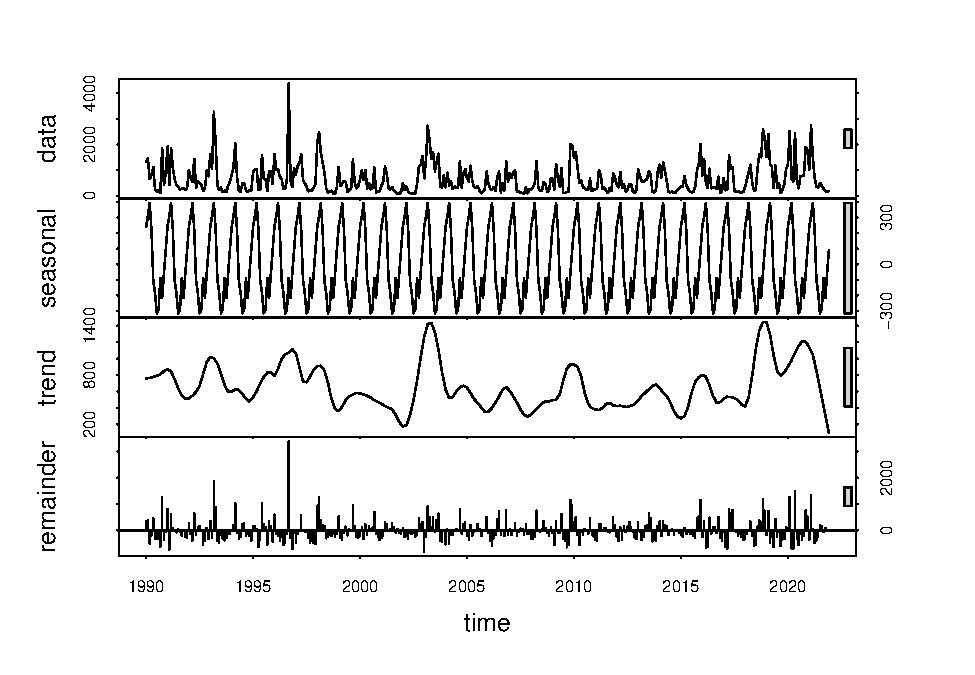
\includegraphics{Project_files/figure-latex/time-series analysis on Regular Water Resources-1.pdf}

\begin{Shaded}
\begin{Highlighting}[]
\NormalTok{CapeFearRiver\_trend }\OtherTok{\textless{}{-}} \FunctionTok{smk.test}\NormalTok{(CapeFearRiver\_timeseries)}
\NormalTok{CapeFearRiver\_trend}
\end{Highlighting}
\end{Shaded}

\begin{verbatim}
## 
##  Seasonal Mann-Kendall trend test (Hirsch-Slack test)
## 
## data:  CapeFearRiver_timeseries
## z = -0.98775, p-value = 0.3233
## alternative hypothesis: true S is not equal to 0
## sample estimates:
##     S  varS 
##  -212 45632
\end{verbatim}

\begin{Shaded}
\begin{Highlighting}[]
\FunctionTok{summary}\NormalTok{(CapeFearRiver\_trend)}
\end{Highlighting}
\end{Shaded}

\begin{verbatim}
## 
##  Seasonal Mann-Kendall trend test (Hirsch-Slack test)
## 
## data: CapeFearRiver_timeseries
## alternative hypothesis: two.sided
## 
## Statistics for individual seasons
## 
## H0
##                      S   varS    tau      z Pr(>|z|)  
## Season 1:   S = 0  -98 3802.7 -0.198 -1.573  0.11572  
## Season 2:   S = 0  -18 3802.7 -0.036 -0.276  0.78279  
## Season 3:   S = 0  -72 3802.7 -0.145 -1.151  0.24958  
## Season 4:   S = 0  -78 3802.7 -0.157 -1.249  0.21179  
## Season 5:   S = 0   32 3802.7  0.065  0.503  0.61517  
## Season 6:   S = 0   24 3802.7  0.048  0.373  0.70916  
## Season 7:   S = 0  -48 3802.7 -0.097 -0.762  0.44596  
## Season 8:   S = 0   24 3802.7  0.048  0.373  0.70916  
## Season 9:   S = 0   12 3802.7  0.024  0.178  0.85842  
## Season 10:   S = 0  -4 3802.7 -0.008 -0.049  0.96120  
## Season 11:   S = 0  -4 3802.7 -0.008 -0.049  0.96120  
## Season 12:   S = 0  18 3802.7  0.036  0.276  0.78279  
## ---
## Signif. codes:  0 '***' 0.001 '**' 0.01 '*' 0.05 '.' 0.1 ' ' 1
\end{verbatim}

\begin{Shaded}
\begin{Highlighting}[]
\CommentTok{\#p{-}value is 0.3233, so there is no trend present in Cape Fear River.}

\NormalTok{FlatRiver\_timeseries }\OtherTok{\textless{}{-}} \FunctionTok{ts}\NormalTok{(FlatRiverDischarge\_Monthly}\SpecialCharTok{$}\NormalTok{Mean\_Flat\_Discharge\_Bymonth, }\AttributeTok{frequency =} \DecValTok{12}\NormalTok{,}
                           \AttributeTok{start =} \FunctionTok{c}\NormalTok{(}\DecValTok{1990}\NormalTok{, }\DecValTok{1}\NormalTok{, }\DecValTok{1}\NormalTok{), }\AttributeTok{end =} \FunctionTok{c}\NormalTok{(}\DecValTok{2021}\NormalTok{, }\DecValTok{12}\NormalTok{, }\DecValTok{1}\NormalTok{))}
\NormalTok{FlatRiver\_Decomposed }\OtherTok{\textless{}{-}} \FunctionTok{stl}\NormalTok{(FlatRiver\_timeseries, }\AttributeTok{s.window =} \StringTok{"periodic"}\NormalTok{)}
\FunctionTok{plot}\NormalTok{(FlatRiver\_Decomposed)}
\end{Highlighting}
\end{Shaded}

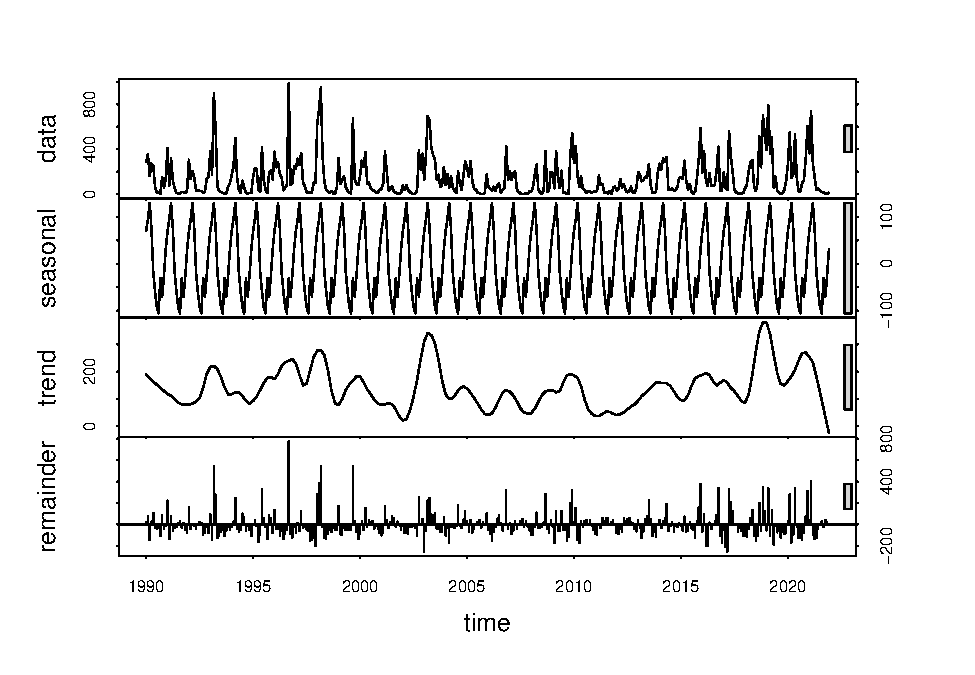
\includegraphics{Project_files/figure-latex/time-series analysis on Regular Water Resources-2.pdf}

\begin{Shaded}
\begin{Highlighting}[]
\NormalTok{FlatRiver\_trend }\OtherTok{\textless{}{-}} \FunctionTok{smk.test}\NormalTok{(FlatRiver\_timeseries)}
\NormalTok{FlatRiver\_trend}
\end{Highlighting}
\end{Shaded}

\begin{verbatim}
## 
##  Seasonal Mann-Kendall trend test (Hirsch-Slack test)
## 
## data:  FlatRiver_timeseries
## z = 0.84731, p-value = 0.3968
## alternative hypothesis: true S is not equal to 0
## sample estimates:
##     S  varS 
##   182 45632
\end{verbatim}

\begin{Shaded}
\begin{Highlighting}[]
\FunctionTok{summary}\NormalTok{(FlatRiver\_trend)}
\end{Highlighting}
\end{Shaded}

\begin{verbatim}
## 
##  Seasonal Mann-Kendall trend test (Hirsch-Slack test)
## 
## data: FlatRiver_timeseries
## alternative hypothesis: two.sided
## 
## Statistics for individual seasons
## 
## H0
##                      S   varS    tau      z Pr(>|z|)  
## Season 1:   S = 0  -76 3802.7 -0.153 -1.216 0.223896  
## Season 2:   S = 0    4 3802.7  0.008  0.049 0.961199  
## Season 3:   S = 0  -92 3802.7 -0.185 -1.476 0.140025  
## Season 4:   S = 0  -18 3802.7 -0.036 -0.276 0.782794  
## Season 5:   S = 0  108 3802.7  0.218  1.735 0.082712 .
## Season 6:   S = 0  110 3802.7  0.222  1.768 0.077129 .
## Season 7:   S = 0   38 3802.7  0.077  0.600 0.548500  
## Season 8:   S = 0   36 3802.7  0.073  0.568 0.570323  
## Season 9:   S = 0   58 3802.7  0.117  0.924 0.355310  
## Season 10:   S = 0 -18 3802.7 -0.036 -0.276 0.782794  
## Season 11:   S = 0   2 3802.7  0.004  0.016 0.987062  
## Season 12:   S = 0  30 3802.7  0.060  0.470 0.638157  
## ---
## Signif. codes:  0 '***' 0.001 '**' 0.01 '*' 0.05 '.' 0.1 ' ' 1
\end{verbatim}

\begin{Shaded}
\begin{Highlighting}[]
\CommentTok{\#p{-}value is 0.3968, so there is no trend present in Flat River.}

\NormalTok{LittleRiver\_timeseries }\OtherTok{\textless{}{-}} \FunctionTok{ts}\NormalTok{(LittleRiverDischarge\_Monthly}\SpecialCharTok{$}\NormalTok{Mean\_Little\_Discharge\_Bymonth, }\AttributeTok{frequency =} \DecValTok{12}\NormalTok{,}
                           \AttributeTok{start =} \FunctionTok{c}\NormalTok{(}\DecValTok{1990}\NormalTok{, }\DecValTok{1}\NormalTok{, }\DecValTok{1}\NormalTok{), }\AttributeTok{end =} \FunctionTok{c}\NormalTok{(}\DecValTok{2021}\NormalTok{, }\DecValTok{12}\NormalTok{, }\DecValTok{1}\NormalTok{))}
\NormalTok{LittleRiver\_Decomposed }\OtherTok{\textless{}{-}} \FunctionTok{stl}\NormalTok{(LittleRiver\_timeseries, }\AttributeTok{s.window =} \StringTok{"periodic"}\NormalTok{)}
\FunctionTok{plot}\NormalTok{(LittleRiver\_Decomposed)}
\end{Highlighting}
\end{Shaded}

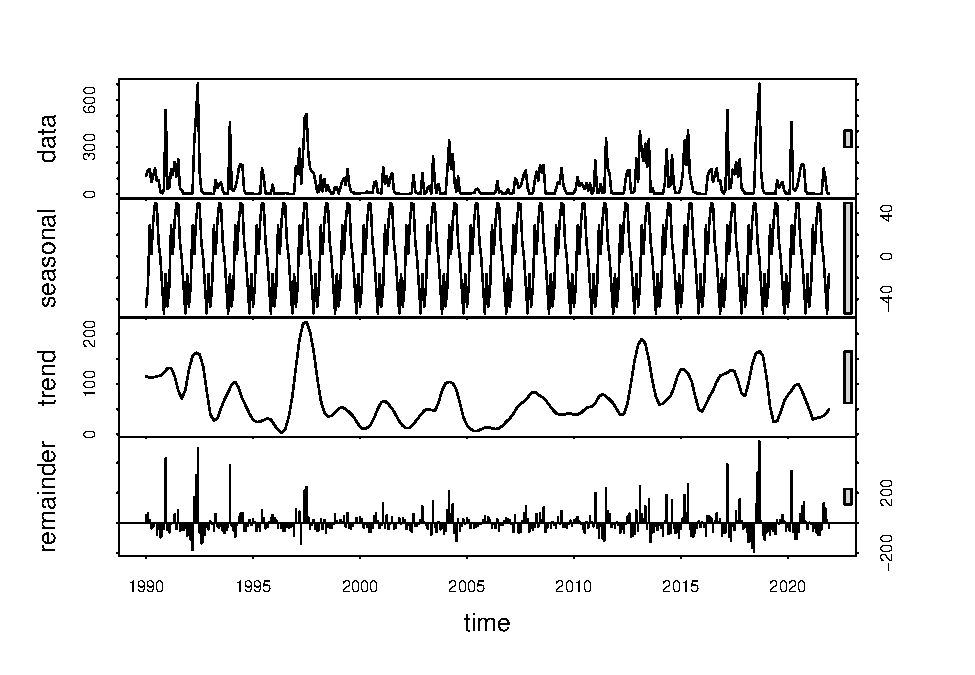
\includegraphics{Project_files/figure-latex/time-series analysis on Regular Water Resources-3.pdf}

\begin{Shaded}
\begin{Highlighting}[]
\NormalTok{LittleRiver\_trend }\OtherTok{\textless{}{-}} \FunctionTok{smk.test}\NormalTok{(LittleRiver\_timeseries)}
\NormalTok{LittleRiver\_trend}
\end{Highlighting}
\end{Shaded}

\begin{verbatim}
## 
##  Seasonal Mann-Kendall trend test (Hirsch-Slack test)
## 
## data:  LittleRiver_timeseries
## z = 0.82859, p-value = 0.4073
## alternative hypothesis: true S is not equal to 0
## sample estimates:
##     S  varS 
##   178 45632
\end{verbatim}

\begin{Shaded}
\begin{Highlighting}[]
\FunctionTok{summary}\NormalTok{(LittleRiver\_trend)}
\end{Highlighting}
\end{Shaded}

\begin{verbatim}
## 
##  Seasonal Mann-Kendall trend test (Hirsch-Slack test)
## 
## data: LittleRiver_timeseries
## alternative hypothesis: two.sided
## 
## Statistics for individual seasons
## 
## H0
##                       S   varS    tau      z  Pr(>|z|)   
## Season 1:   S = 0   -24 3802.7 -0.048 -0.373 0.7091645   
## Season 2:   S = 0   -60 3802.7 -0.121 -0.957 0.3386830   
## Season 3:   S = 0   -16 3802.7 -0.032 -0.243 0.8078142   
## Season 4:   S = 0   -72 3802.7 -0.145 -1.151 0.2495808   
## Season 5:   S = 0   -76 3802.7 -0.153 -1.216 0.2238958   
## Season 6:   S = 0  -120 3802.7 -0.242 -1.930 0.0536368  .
## Season 7:   S = 0   -18 3802.7 -0.036 -0.276 0.7827941   
## Season 8:   S = 0    94 3802.7  0.190  1.508 0.1315212   
## Season 9:   S = 0   202 3802.7  0.407  3.260 0.0011161 **
## Season 10:   S = 0  194 3802.7  0.391  3.130 0.0017494 **
## Season 11:   S = 0  126 3802.7  0.254  2.027 0.0426566  *
## Season 12:   S = 0  -52 3802.7 -0.105 -0.827 0.4082149   
## ---
## Signif. codes:  0 '***' 0.001 '**' 0.01 '*' 0.05 '.' 0.1 ' ' 1
\end{verbatim}

\begin{Shaded}
\begin{Highlighting}[]
\CommentTok{\#p{-}value is 0.4073, so there is no trend present in Little River.}
\CommentTok{\#The time{-}series analysis on Cape Fear Lake, Flat River and Little River do not show any obvious trend in long term. However, we can tell a great similarity between the trend patterns of Cape Fear Lake and Flat River. This raises our concern because they do not come from the same basin. Instead, Little River, which comes from the same watershed as Flat River, shows a more different pattern.}
\end{Highlighting}
\end{Shaded}

\begin{Shaded}
\begin{Highlighting}[]
\CommentTok{\#Total Withdrawals}
\NormalTok{total\_withdrawal\_timeseries }\OtherTok{\textless{}{-}} \FunctionTok{ts}\NormalTok{(total\_withdrawal}\SpecialCharTok{$}\NormalTok{Avg\_Daily\_Use\_mgd, }\AttributeTok{frequency =} \DecValTok{12}\NormalTok{,}
                           \AttributeTok{start =} \FunctionTok{c}\NormalTok{(}\DecValTok{2006}\NormalTok{, }\DecValTok{1}\NormalTok{, }\DecValTok{1}\NormalTok{), }\AttributeTok{end =} \FunctionTok{c}\NormalTok{(}\DecValTok{2021}\NormalTok{, }\DecValTok{12}\NormalTok{, }\DecValTok{1}\NormalTok{))}
\NormalTok{total\_withdrawal\_Decomposed }\OtherTok{\textless{}{-}} \FunctionTok{stl}\NormalTok{(total\_withdrawal\_timeseries, }\AttributeTok{s.window =} \StringTok{"periodic"}\NormalTok{)}
\FunctionTok{plot}\NormalTok{(total\_withdrawal\_Decomposed)}
\end{Highlighting}
\end{Shaded}

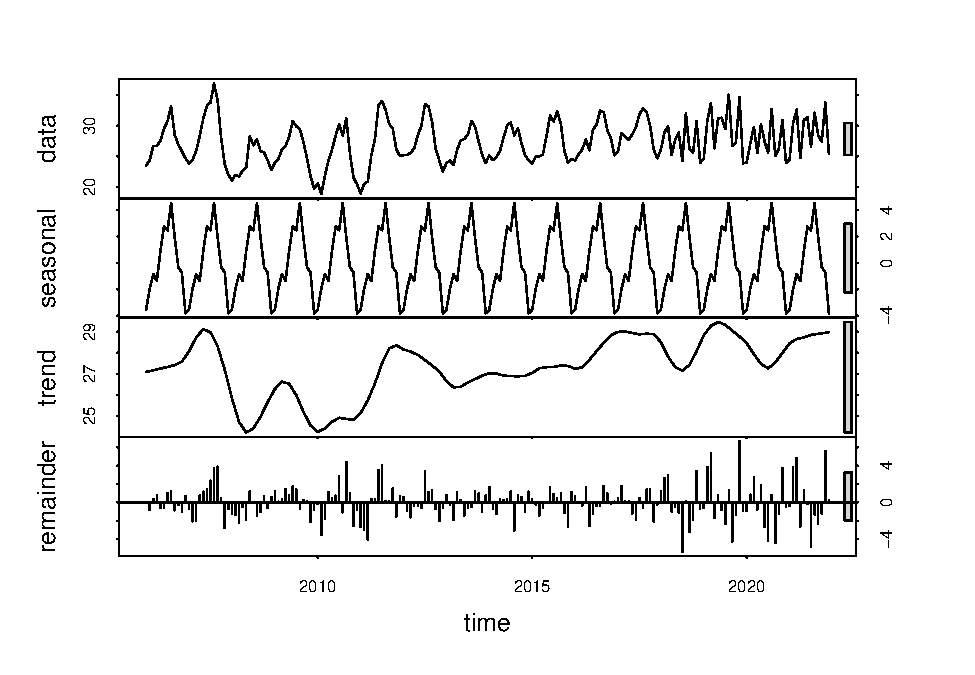
\includegraphics{Project_files/figure-latex/time-series analysis on withdrawals-1.pdf}

\begin{Shaded}
\begin{Highlighting}[]
\NormalTok{total\_withdrawal\_trend }\OtherTok{\textless{}{-}} \FunctionTok{smk.test}\NormalTok{(total\_withdrawal\_timeseries)}
\NormalTok{total\_withdrawal\_trend}
\end{Highlighting}
\end{Shaded}

\begin{verbatim}
## 
##  Seasonal Mann-Kendall trend test (Hirsch-Slack test)
## 
## data:  total_withdrawal_timeseries
## z = 3.5874, p-value = 0.0003339
## alternative hypothesis: true S is not equal to 0
## sample estimates:
##    S varS 
##  277 5919
\end{verbatim}

\begin{Shaded}
\begin{Highlighting}[]
\FunctionTok{summary}\NormalTok{(total\_withdrawal\_trend)}
\end{Highlighting}
\end{Shaded}

\begin{verbatim}
## 
##  Seasonal Mann-Kendall trend test (Hirsch-Slack test)
## 
## data: total_withdrawal_timeseries
## alternative hypothesis: two.sided
## 
## Statistics for individual seasons
## 
## H0
##                      S  varS    tau      z   Pr(>|z|)    
## Season 1:   S = 0   48 493.3  0.400  2.116 0.03433985   *
## Season 2:   S = 0   75 492.3  0.628  3.335 0.00085285 ***
## Season 3:   S = 0   56 493.3  0.467  2.476 0.01327749   *
## Season 4:   S = 0  -12 493.3 -0.100 -0.495 0.62042529    
## Season 5:   S = 0   40 493.3  0.333  1.756 0.07910922   .
## Season 6:   S = 0   -6 493.3 -0.050 -0.225 0.82189169    
## Season 7:   S = 0  -40 493.3 -0.333 -1.756 0.07910922   .
## Season 8:   S = 0   14 493.3  0.117  0.585 0.55835091    
## Season 9:   S = 0  -18 493.3 -0.150 -0.765 0.44404364    
## Season 10:   S = 0  14 493.3  0.117  0.585 0.55835091    
## Season 11:   S = 0  70 493.3  0.583  3.107 0.00189282  **
## Season 12:   S = 0  36 493.3  0.300  1.576 0.11507465    
## ---
## Signif. codes:  0 '***' 0.001 '**' 0.01 '*' 0.05 '.' 0.1 ' ' 1
\end{verbatim}

\begin{Shaded}
\begin{Highlighting}[]
\CommentTok{\#p{-}value is 0.3775, so there is no trend present in Total Withdrawals.}
\CommentTok{\#The time{-}series analysis on municipal withdrawals in Durham shows an obvious increase since 2010. However, the drop in 2019 and 2021 needs more data and reports to explain. }
\end{Highlighting}
\end{Shaded}

\begin{Shaded}
\begin{Highlighting}[]
\NormalTok{DurhamGroundwater\_timeseries }\OtherTok{\textless{}{-}} \FunctionTok{ts}\NormalTok{(DurhamGroundwater}\SpecialCharTok{$}\NormalTok{Groundwater\_Table\_feet, }\AttributeTok{frequency =} \DecValTok{12}\NormalTok{,}
                           \AttributeTok{start =} \FunctionTok{c}\NormalTok{(}\DecValTok{2009}\NormalTok{, }\DecValTok{1}\NormalTok{, }\DecValTok{1}\NormalTok{), }\AttributeTok{end =} \FunctionTok{c}\NormalTok{(}\DecValTok{2021}\NormalTok{, }\DecValTok{12}\NormalTok{, }\DecValTok{1}\NormalTok{))}
\NormalTok{DurhamGroundwater\_Decomposed }\OtherTok{\textless{}{-}} \FunctionTok{stl}\NormalTok{(DurhamGroundwater\_timeseries, }\AttributeTok{s.window =} \StringTok{"periodic"}\NormalTok{)}
\FunctionTok{plot}\NormalTok{(DurhamGroundwater\_Decomposed)}
\end{Highlighting}
\end{Shaded}

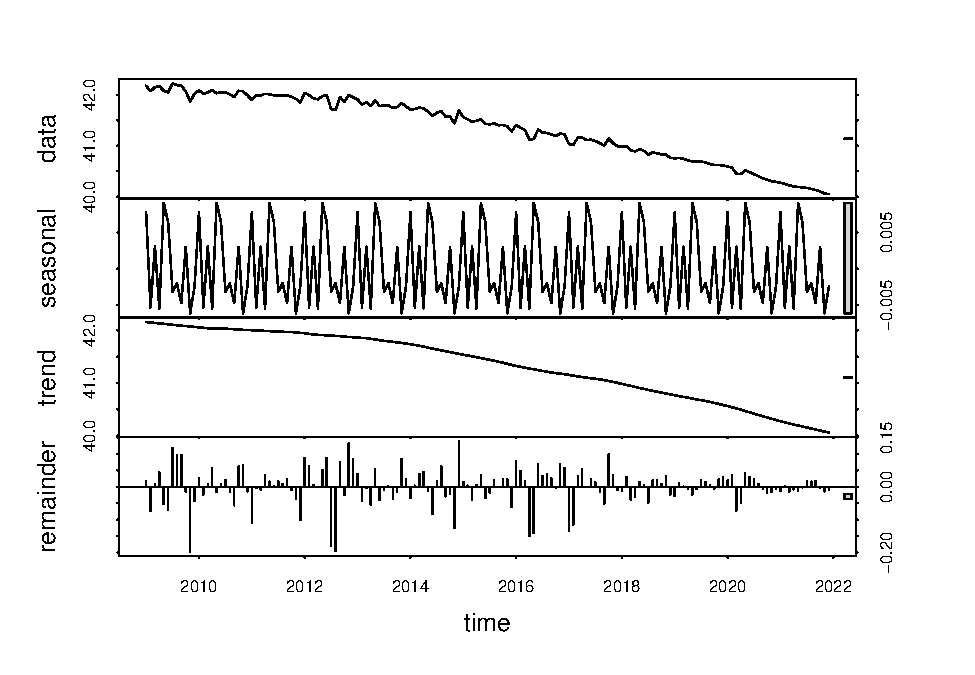
\includegraphics{Project_files/figure-latex/time-series analysis on groundwater-1.pdf}

\begin{Shaded}
\begin{Highlighting}[]
\NormalTok{DurhamGroundwater\_trend }\OtherTok{\textless{}{-}} \FunctionTok{smk.test}\NormalTok{(DurhamGroundwater\_timeseries)}
\NormalTok{DurhamGroundwater\_trend}
\end{Highlighting}
\end{Shaded}

\begin{verbatim}
## 
##  Seasonal Mann-Kendall trend test (Hirsch-Slack test)
## 
## data:  DurhamGroundwater_timeseries
## z = -15.964, p-value < 2.2e-16
## alternative hypothesis: true S is not equal to 0
## sample estimates:
##    S varS 
## -907 3221
\end{verbatim}

\begin{Shaded}
\begin{Highlighting}[]
\FunctionTok{summary}\NormalTok{(DurhamGroundwater\_trend)}
\end{Highlighting}
\end{Shaded}

\begin{verbatim}
## 
##  Seasonal Mann-Kendall trend test (Hirsch-Slack test)
## 
## data: DurhamGroundwater_timeseries
## alternative hypothesis: two.sided
## 
## Statistics for individual seasons
## 
## H0
##                      S  varS    tau      z   Pr(>|z|)    
## Season 1:   S = 0  -74 268.7 -0.949 -4.454 8.4423e-06 ***
## Season 2:   S = 0  -77 267.7 -0.994 -4.645 3.3954e-06 ***
## Season 3:   S = 0  -78 268.7 -1.000 -4.698 2.6313e-06 ***
## Season 4:   S = 0  -76 268.7 -0.974 -4.576 4.7471e-06 ***
## Season 5:   S = 0  -78 268.7 -1.000 -4.698 2.6313e-06 ***
## Season 6:   S = 0  -75 267.7 -0.968 -4.523 6.0945e-06 ***
## Season 7:   S = 0  -76 268.7 -0.974 -4.576 4.7471e-06 ***
## Season 8:   S = 0  -76 268.7 -0.974 -4.576 4.7471e-06 ***
## Season 9:   S = 0  -75 267.7 -0.968 -4.523 6.0945e-06 ***
## Season 10:   S = 0 -76 268.7 -0.974 -4.576 4.7471e-06 ***
## Season 11:   S = 0 -70 268.7 -0.897 -4.210 2.5581e-05 ***
## Season 12:   S = 0 -76 268.7 -0.974 -4.576 4.7471e-06 ***
## ---
## Signif. codes:  0 '***' 0.001 '**' 0.01 '*' 0.05 '.' 0.1 ' ' 1
\end{verbatim}

\begin{Shaded}
\begin{Highlighting}[]
\CommentTok{\#p{-}value is less than 0.05, so there is no trend present in Total Withdrawals.}
\CommentTok{\#The time{-}series analysis on groundwater table level in Durham shows a significant decrease since 2010. }
\end{Highlighting}
\end{Shaded}

\begin{Shaded}
\begin{Highlighting}[]
\NormalTok{DurhamPrecipitaion\_timeseries }\OtherTok{\textless{}{-}} \FunctionTok{ts}\NormalTok{(DurhamPrecipitaion}\SpecialCharTok{$}\NormalTok{Precipitaion\_inches, }\AttributeTok{frequency =} \DecValTok{12}\NormalTok{,}
                           \AttributeTok{start =} \FunctionTok{c}\NormalTok{(}\DecValTok{2009}\NormalTok{, }\DecValTok{1}\NormalTok{, }\DecValTok{1}\NormalTok{), }\AttributeTok{end =} \FunctionTok{c}\NormalTok{(}\DecValTok{2021}\NormalTok{, }\DecValTok{12}\NormalTok{, }\DecValTok{1}\NormalTok{))}
\NormalTok{DurhamPrecipitaion\_Decomposed }\OtherTok{\textless{}{-}} \FunctionTok{stl}\NormalTok{(DurhamPrecipitaion\_timeseries, }\AttributeTok{s.window =} \StringTok{"periodic"}\NormalTok{)}
\FunctionTok{plot}\NormalTok{(DurhamPrecipitaion\_Decomposed)}
\end{Highlighting}
\end{Shaded}

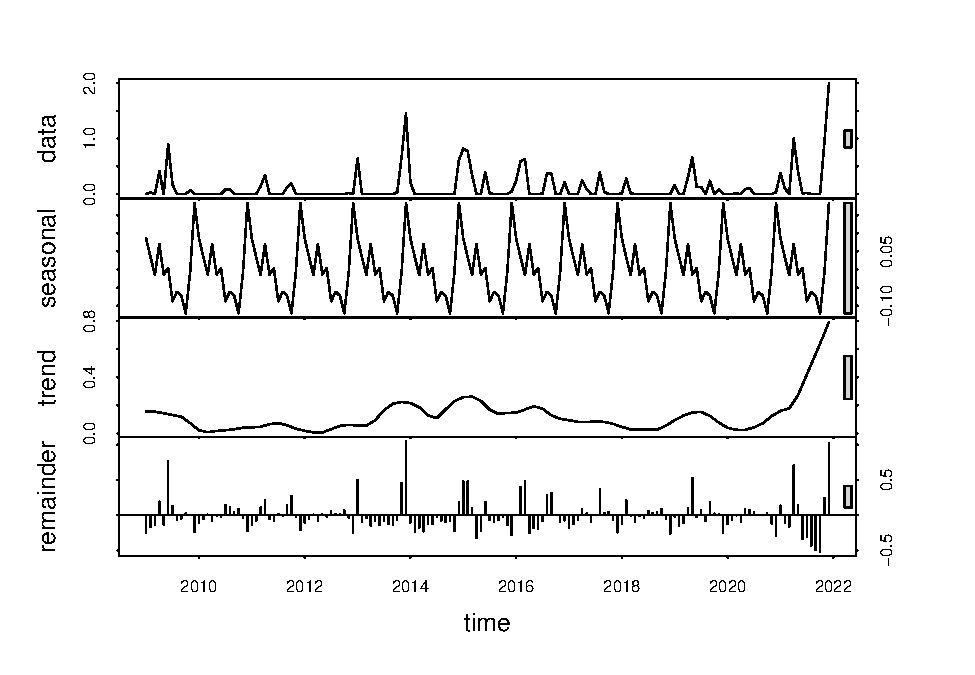
\includegraphics{Project_files/figure-latex/time-series analysis on precipitation-1.pdf}

\begin{Shaded}
\begin{Highlighting}[]
\NormalTok{DurhamPrecipitaion\_trend }\OtherTok{\textless{}{-}} \FunctionTok{smk.test}\NormalTok{(DurhamGroundwater\_timeseries)}
\NormalTok{DurhamPrecipitaion\_trend}
\end{Highlighting}
\end{Shaded}

\begin{verbatim}
## 
##  Seasonal Mann-Kendall trend test (Hirsch-Slack test)
## 
## data:  DurhamGroundwater_timeseries
## z = -15.964, p-value < 2.2e-16
## alternative hypothesis: true S is not equal to 0
## sample estimates:
##    S varS 
## -907 3221
\end{verbatim}

\begin{Shaded}
\begin{Highlighting}[]
\FunctionTok{summary}\NormalTok{(DurhamPrecipitaion\_trend)}
\end{Highlighting}
\end{Shaded}

\begin{verbatim}
## 
##  Seasonal Mann-Kendall trend test (Hirsch-Slack test)
## 
## data: DurhamGroundwater_timeseries
## alternative hypothesis: two.sided
## 
## Statistics for individual seasons
## 
## H0
##                      S  varS    tau      z   Pr(>|z|)    
## Season 1:   S = 0  -74 268.7 -0.949 -4.454 8.4423e-06 ***
## Season 2:   S = 0  -77 267.7 -0.994 -4.645 3.3954e-06 ***
## Season 3:   S = 0  -78 268.7 -1.000 -4.698 2.6313e-06 ***
## Season 4:   S = 0  -76 268.7 -0.974 -4.576 4.7471e-06 ***
## Season 5:   S = 0  -78 268.7 -1.000 -4.698 2.6313e-06 ***
## Season 6:   S = 0  -75 267.7 -0.968 -4.523 6.0945e-06 ***
## Season 7:   S = 0  -76 268.7 -0.974 -4.576 4.7471e-06 ***
## Season 8:   S = 0  -76 268.7 -0.974 -4.576 4.7471e-06 ***
## Season 9:   S = 0  -75 267.7 -0.968 -4.523 6.0945e-06 ***
## Season 10:   S = 0 -76 268.7 -0.974 -4.576 4.7471e-06 ***
## Season 11:   S = 0 -70 268.7 -0.897 -4.210 2.5581e-05 ***
## Season 12:   S = 0 -76 268.7 -0.974 -4.576 4.7471e-06 ***
## ---
## Signif. codes:  0 '***' 0.001 '**' 0.01 '*' 0.05 '.' 0.1 ' ' 1
\end{verbatim}

\begin{Shaded}
\begin{Highlighting}[]
\CommentTok{\#The time{-}series analysis on precipitation in Durham shows a gradual rise since 2010 and a dynamic increase in recent years. }
\end{Highlighting}
\end{Shaded}

\begin{Shaded}
\begin{Highlighting}[]
\NormalTok{precip }\OtherTok{\textless{}{-}}\NormalTok{ DurhamPrecipitaion }\SpecialCharTok{\%\textgreater{}\%}
  \FunctionTok{select}\NormalTok{(Date, Precipitaion\_inches) }\SpecialCharTok{\%\textgreater{}\%}
  \FunctionTok{filter}\NormalTok{(Date }\SpecialCharTok{\textgreater{}} \StringTok{"2013{-}12{-}31"}\NormalTok{)}
\NormalTok{capefear }\OtherTok{\textless{}{-}}\NormalTok{ CapeFearRiverDischarge }\SpecialCharTok{\%\textgreater{}\%}
  \FunctionTok{select}\NormalTok{(Date, CapeFear\_Discharge) }\SpecialCharTok{\%\textgreater{}\%}
  \FunctionTok{filter}\NormalTok{(Date }\SpecialCharTok{\textgreater{}} \StringTok{"2013{-}12{-}31"}\NormalTok{)}
\NormalTok{flat }\OtherTok{\textless{}{-}}\NormalTok{ FlatRiverDischarge }\SpecialCharTok{\%\textgreater{}\%}
  \FunctionTok{select}\NormalTok{(Date, Flat\_Discharge) }\SpecialCharTok{\%\textgreater{}\%}
  \FunctionTok{filter}\NormalTok{(Date }\SpecialCharTok{\textgreater{}} \StringTok{"2013{-}12{-}31"}\NormalTok{)}
\NormalTok{little }\OtherTok{\textless{}{-}}\NormalTok{ LittleRiverDischarge }\SpecialCharTok{\%\textgreater{}\%}
  \FunctionTok{select}\NormalTok{(Date, Little\_Discharge) }\SpecialCharTok{\%\textgreater{}\%}
  \FunctionTok{filter}\NormalTok{(Date }\SpecialCharTok{\textgreater{}} \StringTok{"2013{-}12{-}31"}\NormalTok{)}
\NormalTok{data1 }\OtherTok{\textless{}{-}} \FunctionTok{left\_join}\NormalTok{(precip, capefear) }\SpecialCharTok{\%\textgreater{}\%}
  \FunctionTok{left\_join}\NormalTok{(., flat) }\SpecialCharTok{\%\textgreater{}\%}
  \FunctionTok{left\_join}\NormalTok{(., little) }
\end{Highlighting}
\end{Shaded}

\begin{verbatim}
## Joining, by = "Date"
## Joining, by = "Date"
## Joining, by = "Date"
\end{verbatim}

\begin{Shaded}
\begin{Highlighting}[]
\NormalTok{mod1 }\OtherTok{\textless{}{-}} \FunctionTok{lm}\NormalTok{(Precipitaion\_inches }\SpecialCharTok{\textasciitilde{}}\NormalTok{ CapeFear\_Discharge }\SpecialCharTok{+}\NormalTok{ Flat\_Discharge }\SpecialCharTok{+}\NormalTok{ Little\_Discharge, }\AttributeTok{data =}\NormalTok{ data1)}
\FunctionTok{summary}\NormalTok{(mod1)}
\end{Highlighting}
\end{Shaded}

\begin{verbatim}
## 
## Call:
## lm(formula = Precipitaion_inches ~ CapeFear_Discharge + Flat_Discharge + 
##     Little_Discharge, data = data1)
## 
## Residuals:
##     Min      1Q  Median      3Q     Max 
## -2.0634 -0.1224 -0.1047 -0.0677  4.8682 
## 
## Coefficients:
##                      Estimate Std. Error t value Pr(>|t|)    
## (Intercept)         1.041e-01  8.138e-03  12.792  < 2e-16 ***
## CapeFear_Discharge -4.799e-05  8.167e-06  -5.877 4.67e-09 ***
## Flat_Discharge      4.917e-04  4.258e-05  11.547  < 2e-16 ***
## Little_Discharge   -1.576e-04  5.873e-05  -2.683  0.00734 ** 
## ---
## Signif. codes:  0 '***' 0.001 '**' 0.01 '*' 0.05 '.' 0.1 ' ' 1
## 
## Residual standard error: 0.3848 on 2869 degrees of freedom
##   (12 observations deleted due to missingness)
## Multiple R-squared:  0.1374, Adjusted R-squared:  0.1365 
## F-statistic: 152.4 on 3 and 2869 DF,  p-value: < 2.2e-16
\end{verbatim}

\begin{Shaded}
\begin{Highlighting}[]
\FunctionTok{par}\NormalTok{(}\AttributeTok{mfrow=}\FunctionTok{c}\NormalTok{(}\DecValTok{2}\NormalTok{,}\DecValTok{2}\NormalTok{))}
\FunctionTok{plot}\NormalTok{(mod1)}
\end{Highlighting}
\end{Shaded}

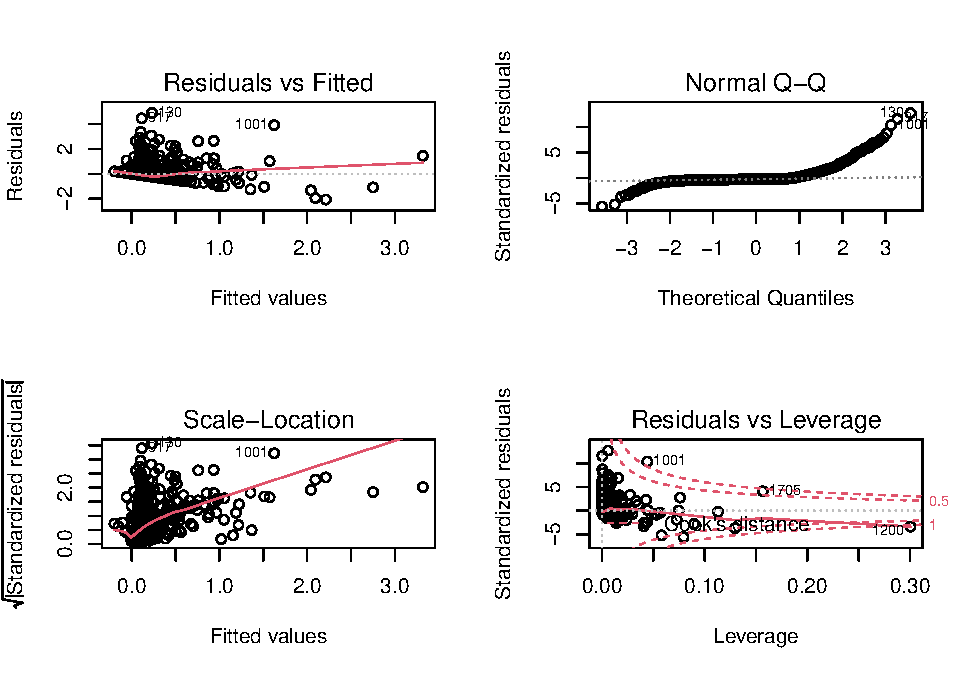
\includegraphics{Project_files/figure-latex/river discharge and precipitation-1.pdf}

\begin{Shaded}
\begin{Highlighting}[]
\NormalTok{totalwit }\OtherTok{\textless{}{-}}\NormalTok{ total\_withdrawal\_Monthly }\SpecialCharTok{\%\textgreater{}\%}
  \FunctionTok{select}\NormalTok{(Month, Mean\_Avg\_Daily\_Use\_mgd) }\SpecialCharTok{\%\textgreater{}\%}
  \FunctionTok{filter}\NormalTok{(Month }\SpecialCharTok{\textgreater{}} \StringTok{"2013{-}12"}\NormalTok{) }
\NormalTok{capefearmonthly }\OtherTok{\textless{}{-}}\NormalTok{ CapeFearRiverDischarge\_Monthly }\SpecialCharTok{\%\textgreater{}\%}
  \FunctionTok{select}\NormalTok{(Month, Mean\_CapeFear\_Discharge\_Bymonth) }\SpecialCharTok{\%\textgreater{}\%}
  \FunctionTok{filter}\NormalTok{(Month }\SpecialCharTok{\textgreater{}} \StringTok{"2013{-}12"}\NormalTok{) }\SpecialCharTok{\%\textgreater{}\%}
  \FunctionTok{mutate}\NormalTok{(}\AttributeTok{CapeFear\_Discharge =}\NormalTok{ Mean\_CapeFear\_Discharge\_Bymonth)}
\NormalTok{flatmonthly }\OtherTok{\textless{}{-}}\NormalTok{ FlatRiverDischarge\_Monthly }\SpecialCharTok{\%\textgreater{}\%}
  \FunctionTok{select}\NormalTok{(Month, Mean\_Flat\_Discharge\_Bymonth) }\SpecialCharTok{\%\textgreater{}\%}
  \FunctionTok{filter}\NormalTok{(Month }\SpecialCharTok{\textgreater{}} \StringTok{"2013{-}12"}\NormalTok{) }\SpecialCharTok{\%\textgreater{}\%}
  \FunctionTok{mutate}\NormalTok{(}\AttributeTok{Flat\_Discharge =}\NormalTok{ Mean\_Flat\_Discharge\_Bymonth)}
\NormalTok{littlemonthly }\OtherTok{\textless{}{-}}\NormalTok{ LittleRiverDischarge\_Monthly }\SpecialCharTok{\%\textgreater{}\%}
  \FunctionTok{select}\NormalTok{(Month, Mean\_Little\_Discharge\_Bymonth) }\SpecialCharTok{\%\textgreater{}\%}
  \FunctionTok{filter}\NormalTok{(Month }\SpecialCharTok{\textgreater{}} \StringTok{"2013{-}12"}\NormalTok{) }\SpecialCharTok{\%\textgreater{}\%}
  \FunctionTok{mutate}\NormalTok{(}\AttributeTok{Little\_Discharge =}\NormalTok{ Mean\_Little\_Discharge\_Bymonth)}
\NormalTok{data2 }\OtherTok{\textless{}{-}} \FunctionTok{left\_join}\NormalTok{(totalwit, capefearmonthly) }\SpecialCharTok{\%\textgreater{}\%}
  \FunctionTok{left\_join}\NormalTok{(., flatmonthly) }\SpecialCharTok{\%\textgreater{}\%}
  \FunctionTok{left\_join}\NormalTok{(., littlemonthly) }
\end{Highlighting}
\end{Shaded}

\begin{verbatim}
## Joining, by = "Month"
## Joining, by = "Month"
## Joining, by = "Month"
\end{verbatim}

\begin{Shaded}
\begin{Highlighting}[]
\NormalTok{mod2}\FloatTok{.1} \OtherTok{\textless{}{-}} \FunctionTok{lm}\NormalTok{(Mean\_Avg\_Daily\_Use\_mgd }\SpecialCharTok{\textasciitilde{}}\NormalTok{ CapeFear\_Discharge }\SpecialCharTok{+}\NormalTok{ Flat\_Discharge }\SpecialCharTok{+}\NormalTok{ Little\_Discharge, }\AttributeTok{data =}\NormalTok{ data2)}
\FunctionTok{summary}\NormalTok{(mod2}\FloatTok{.1}\NormalTok{)}
\end{Highlighting}
\end{Shaded}

\begin{verbatim}
## 
## Call:
## lm(formula = Mean_Avg_Daily_Use_mgd ~ CapeFear_Discharge + Flat_Discharge + 
##     Little_Discharge, data = data2)
## 
## Residuals:
##     Min      1Q  Median      3Q     Max 
## -4.7101 -2.6601 -0.4312  2.3640  6.3019 
## 
## Coefficients:
##                     Estimate Std. Error t value Pr(>|t|)    
## (Intercept)        28.525224   0.469178  60.798   <2e-16 ***
## CapeFear_Discharge  0.001259   0.001101   1.144   0.2557    
## Flat_Discharge     -0.012179   0.006165  -1.976   0.0512 .  
## Little_Discharge    0.010286   0.008614   1.194   0.2355    
## ---
## Signif. codes:  0 '***' 0.001 '**' 0.01 '*' 0.05 '.' 0.1 ' ' 1
## 
## Residual standard error: 2.959 on 92 degrees of freedom
## Multiple R-squared:  0.06156,    Adjusted R-squared:  0.03096 
## F-statistic: 2.012 on 3 and 92 DF,  p-value: 0.1178
\end{verbatim}

\begin{Shaded}
\begin{Highlighting}[]
\NormalTok{mod2}\FloatTok{.2} \OtherTok{\textless{}{-}} \FunctionTok{update}\NormalTok{(mod2}\FloatTok{.1}\NormalTok{, .}\SpecialCharTok{\textasciitilde{}}\NormalTok{. }\SpecialCharTok{{-}}\NormalTok{CapeFear\_Discharge)}
\FunctionTok{summary}\NormalTok{(mod2}\FloatTok{.2}\NormalTok{)}
\end{Highlighting}
\end{Shaded}

\begin{verbatim}
## 
## Call:
## lm(formula = Mean_Avg_Daily_Use_mgd ~ Flat_Discharge + Little_Discharge, 
##     data = data2)
## 
## Residuals:
##     Min      1Q  Median      3Q     Max 
## -4.5201 -2.6643 -0.3608  2.1502  6.3973 
## 
## Coefficients:
##                   Estimate Std. Error t value Pr(>|t|)    
## (Intercept)      28.732216   0.433587  66.266   <2e-16 ***
## Flat_Discharge   -0.007467   0.004594  -1.625    0.107    
## Little_Discharge  0.008746   0.008522   1.026    0.307    
## ---
## Signif. codes:  0 '***' 0.001 '**' 0.01 '*' 0.05 '.' 0.1 ' ' 1
## 
## Residual standard error: 2.964 on 93 degrees of freedom
## Multiple R-squared:  0.04821,    Adjusted R-squared:  0.02774 
## F-statistic: 2.355 on 2 and 93 DF,  p-value: 0.1005
\end{verbatim}

\begin{Shaded}
\begin{Highlighting}[]
\NormalTok{mod2}\FloatTok{.3} \OtherTok{\textless{}{-}} \FunctionTok{update}\NormalTok{(mod2}\FloatTok{.2}\NormalTok{, .}\SpecialCharTok{\textasciitilde{}}\NormalTok{. }\SpecialCharTok{{-}}\NormalTok{Little\_Discharge)}
\FunctionTok{summary}\NormalTok{(mod2}\FloatTok{.3}\NormalTok{)}
\end{Highlighting}
\end{Shaded}

\begin{verbatim}
## 
## Call:
## lm(formula = Mean_Avg_Daily_Use_mgd ~ Flat_Discharge, data = data2)
## 
## Residuals:
##    Min     1Q Median     3Q    Max 
## -4.436 -2.550 -0.253  2.222  6.489 
## 
## Coefficients:
##                 Estimate Std. Error t value Pr(>|t|)    
## (Intercept)    28.611617   0.417476  68.535   <2e-16 ***
## Flat_Discharge -0.003045   0.001593  -1.912   0.0589 .  
## ---
## Signif. codes:  0 '***' 0.001 '**' 0.01 '*' 0.05 '.' 0.1 ' ' 1
## 
## Residual standard error: 2.965 on 94 degrees of freedom
## Multiple R-squared:  0.03743,    Adjusted R-squared:  0.02719 
## F-statistic: 3.656 on 1 and 94 DF,  p-value: 0.05893
\end{verbatim}

\begin{Shaded}
\begin{Highlighting}[]
\FunctionTok{par}\NormalTok{(}\AttributeTok{mfrow=}\FunctionTok{c}\NormalTok{(}\DecValTok{2}\NormalTok{,}\DecValTok{2}\NormalTok{))}
\FunctionTok{plot}\NormalTok{(mod2}\FloatTok{.1}\NormalTok{)}
\end{Highlighting}
\end{Shaded}

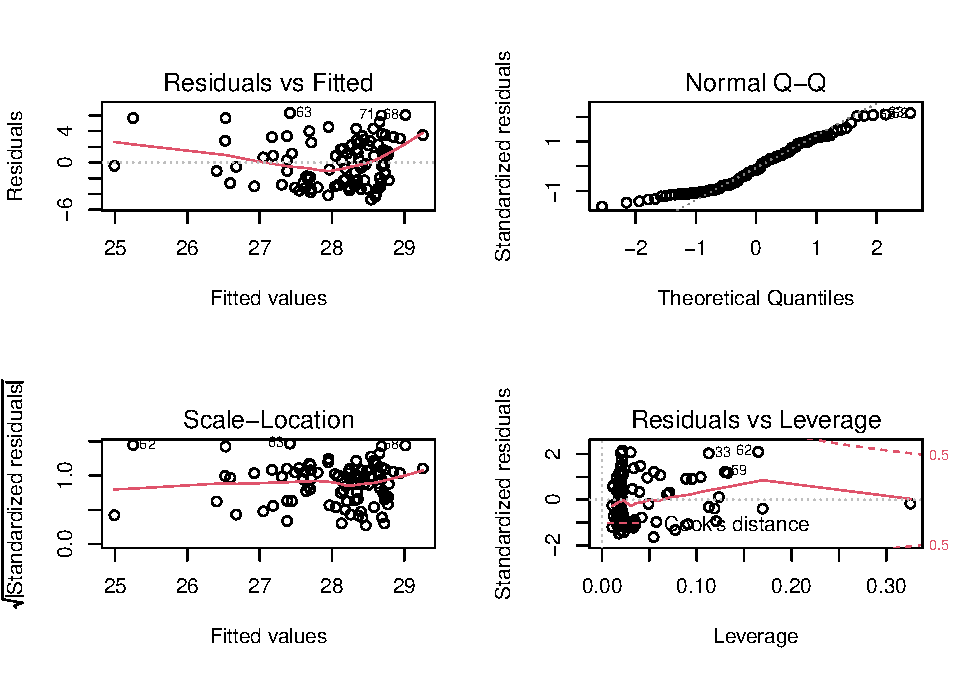
\includegraphics{Project_files/figure-latex/river discharge and withdraws-1.pdf}

\begin{Shaded}
\begin{Highlighting}[]
\NormalTok{precip }\OtherTok{\textless{}{-}}\NormalTok{ DurhamPrecipitaion }\SpecialCharTok{\%\textgreater{}\%}
  \FunctionTok{select}\NormalTok{(Date, Precipitaion\_inches) }\SpecialCharTok{\%\textgreater{}\%}
  \FunctionTok{filter}\NormalTok{(Date }\SpecialCharTok{\textgreater{}} \StringTok{"2013{-}12{-}31"}\NormalTok{)}
\NormalTok{groudw }\OtherTok{\textless{}{-}}\NormalTok{ DurhamGroundwater }\SpecialCharTok{\%\textgreater{}\%}
  \FunctionTok{select}\NormalTok{(Date, Groundwater\_Table\_feet) }\SpecialCharTok{\%\textgreater{}\%}
  \FunctionTok{filter}\NormalTok{(Date }\SpecialCharTok{\textgreater{}} \StringTok{"2013{-}12{-}31"}\NormalTok{)}
\NormalTok{data3 }\OtherTok{\textless{}{-}} \FunctionTok{left\_join}\NormalTok{(groudw, precip)}
\end{Highlighting}
\end{Shaded}

\begin{verbatim}
## Joining, by = "Date"
\end{verbatim}

\begin{Shaded}
\begin{Highlighting}[]
\NormalTok{mod3 }\OtherTok{\textless{}{-}} \FunctionTok{lm}\NormalTok{(Groundwater\_Table\_feet }\SpecialCharTok{\textasciitilde{}}\NormalTok{ Precipitaion\_inches, }\AttributeTok{data =}\NormalTok{ data3)}
\FunctionTok{summary}\NormalTok{(mod3)}
\end{Highlighting}
\end{Shaded}

\begin{verbatim}
## 
## Call:
## lm(formula = Groundwater_Table_feet ~ Precipitaion_inches, data = data3)
## 
## Residuals:
##    Min     1Q Median     3Q    Max 
## -4.830 -1.490  0.396  1.590  3.480 
## 
## Coefficients:
##                     Estimate Std. Error t value Pr(>|t|)    
## (Intercept)         38.74024    0.04274 906.361   <2e-16 ***
## Precipitaion_inches  0.11322    0.09743   1.162    0.245    
## ---
## Signif. codes:  0 '***' 0.001 '**' 0.01 '*' 0.05 '.' 0.1 ' ' 1
## 
## Residual standard error: 2.164 on 2872 degrees of freedom
##   (37 observations deleted due to missingness)
## Multiple R-squared:  0.0004699,  Adjusted R-squared:  0.0001219 
## F-statistic:  1.35 on 1 and 2872 DF,  p-value: 0.2453
\end{verbatim}

\begin{Shaded}
\begin{Highlighting}[]
\FunctionTok{par}\NormalTok{(}\AttributeTok{mfrow=}\FunctionTok{c}\NormalTok{(}\DecValTok{2}\NormalTok{,}\DecValTok{2}\NormalTok{))}
\FunctionTok{plot}\NormalTok{(mod3)}
\end{Highlighting}
\end{Shaded}

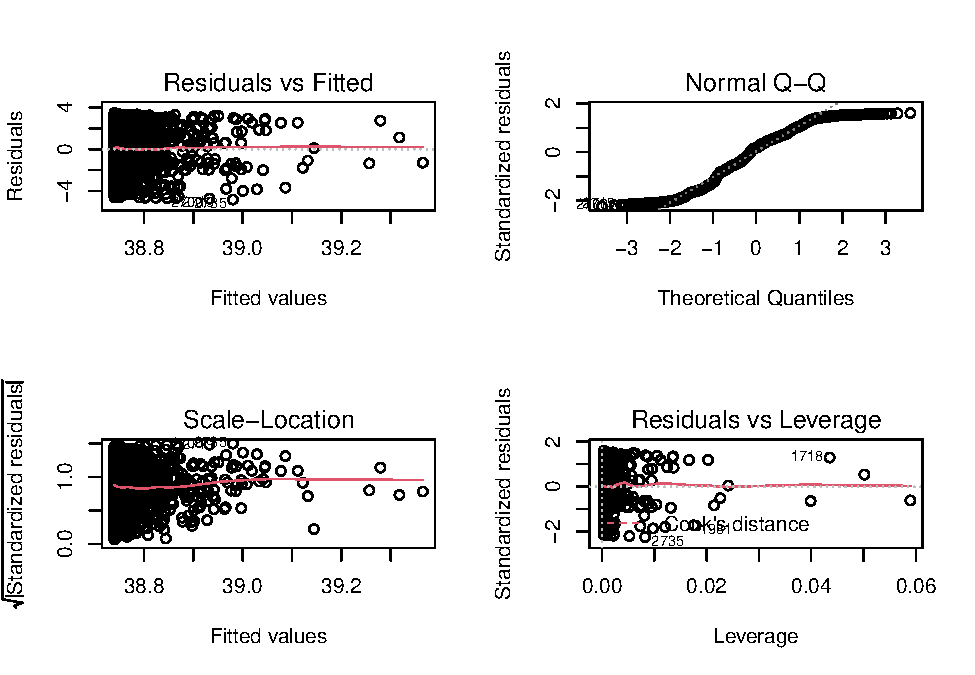
\includegraphics{Project_files/figure-latex/groundwater and precipitation-1.pdf}

\begin{Shaded}
\begin{Highlighting}[]
\NormalTok{totalwit }\OtherTok{\textless{}{-}}\NormalTok{ total\_withdrawal\_Monthly }\SpecialCharTok{\%\textgreater{}\%}
  \FunctionTok{select}\NormalTok{(Month, Mean\_Avg\_Daily\_Use\_mgd) }\SpecialCharTok{\%\textgreater{}\%}
  \FunctionTok{filter}\NormalTok{(Month }\SpecialCharTok{\textgreater{}} \StringTok{"2013{-}12"}\NormalTok{)}
\NormalTok{data4 }\OtherTok{\textless{}{-}} \FunctionTok{left\_join}\NormalTok{(DurhamGroundwater\_Monthly, totalwit) }
\end{Highlighting}
\end{Shaded}

\begin{verbatim}
## Joining, by = "Month"
\end{verbatim}

\begin{Shaded}
\begin{Highlighting}[]
\NormalTok{mod4 }\OtherTok{\textless{}{-}} \FunctionTok{lm}\NormalTok{(Mean\_Groundwater\_Table\_feet }\SpecialCharTok{\textasciitilde{}}\NormalTok{ Mean\_Avg\_Daily\_Use\_mgd, }\AttributeTok{data =}\NormalTok{ data4)}
\FunctionTok{summary}\NormalTok{(mod4)}
\end{Highlighting}
\end{Shaded}

\begin{verbatim}
## 
## Call:
## lm(formula = Mean_Groundwater_Table_feet ~ Mean_Avg_Daily_Use_mgd, 
##     data = data4)
## 
## Residuals:
##     Min      1Q  Median      3Q     Max 
## -4.7842 -1.7200  0.4354  1.5870  4.1540 
## 
## Coefficients:
##                        Estimate Std. Error t value Pr(>|t|)    
## (Intercept)            45.10469    1.99031  22.662  < 2e-16 ***
## Mean_Avg_Daily_Use_mgd -0.22607    0.07053  -3.205  0.00184 ** 
## ---
## Signif. codes:  0 '***' 0.001 '**' 0.01 '*' 0.05 '.' 0.1 ' ' 1
## 
## Residual standard error: 2.067 on 94 degrees of freedom
## Multiple R-squared:  0.09854,    Adjusted R-squared:  0.08895 
## F-statistic: 10.27 on 1 and 94 DF,  p-value: 0.001843
\end{verbatim}

\begin{Shaded}
\begin{Highlighting}[]
\FunctionTok{par}\NormalTok{(}\AttributeTok{mfrow=}\FunctionTok{c}\NormalTok{(}\DecValTok{2}\NormalTok{,}\DecValTok{2}\NormalTok{))}
\FunctionTok{plot}\NormalTok{(mod4)}
\end{Highlighting}
\end{Shaded}

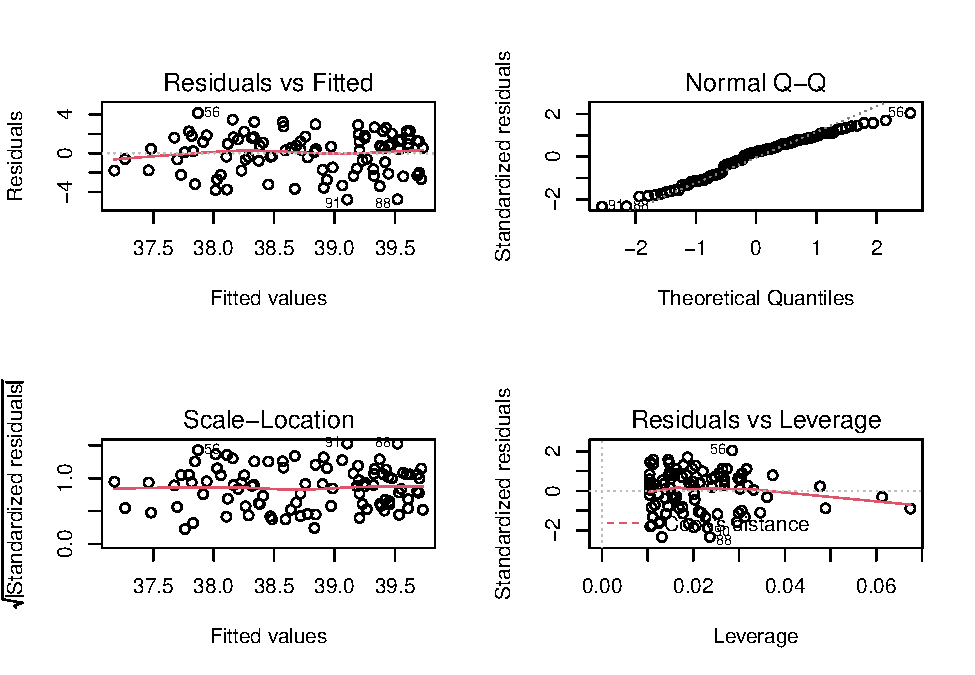
\includegraphics{Project_files/figure-latex/groundwater and withdraws-1.pdf}

\begin{Shaded}
\begin{Highlighting}[]
\FunctionTok{ggplot}\NormalTok{(data4,}\FunctionTok{aes}\NormalTok{(}\AttributeTok{x=}\NormalTok{Mean\_Groundwater\_Table\_feet,}\AttributeTok{y=}\NormalTok{Mean\_Avg\_Daily\_Use\_mgd))}\SpecialCharTok{+}
       \FunctionTok{geom\_point}\NormalTok{()}\SpecialCharTok{+}
  \FunctionTok{theme}\NormalTok{(}\AttributeTok{text =} \FunctionTok{element\_text}\NormalTok{(}\AttributeTok{size =} \DecValTok{19}\NormalTok{))}\SpecialCharTok{+}
  \FunctionTok{geom\_smooth}\NormalTok{(}\AttributeTok{method =}\NormalTok{ lm) }\SpecialCharTok{+}
  \FunctionTok{xlab}\NormalTok{(}\StringTok{"Average Daily Water Use (million gallon/day)"}\NormalTok{)}\SpecialCharTok{+}\FunctionTok{ylab}\NormalTok{(}\StringTok{"Groundwater table (ft)"}\NormalTok{)}
\end{Highlighting}
\end{Shaded}

\begin{verbatim}
## `geom_smooth()` using formula 'y ~ x'
\end{verbatim}

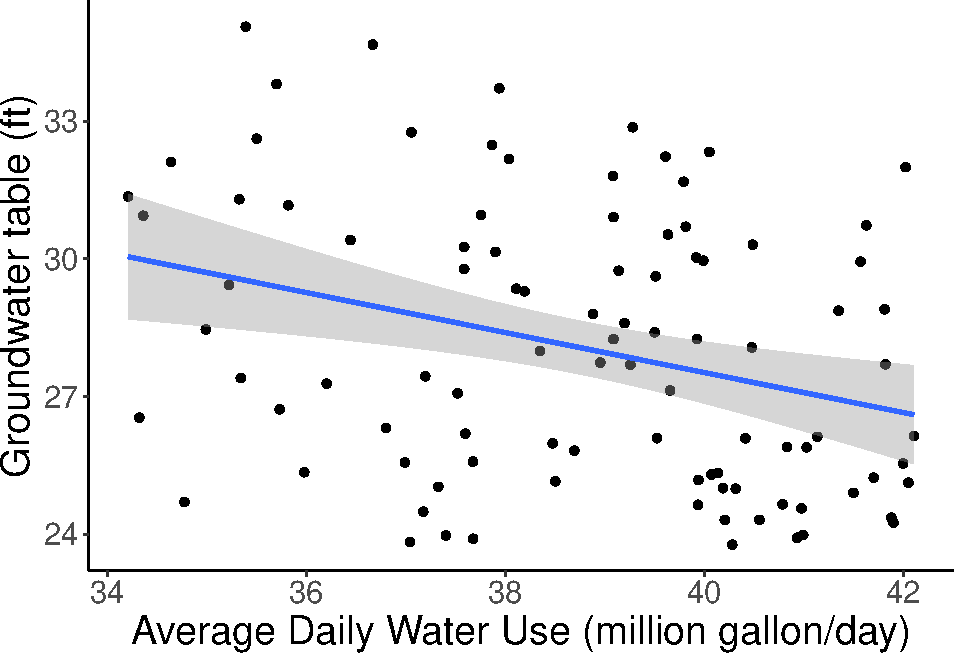
\includegraphics{Project_files/figure-latex/groundwater and withdraws-2.pdf}

\begin{Shaded}
\begin{Highlighting}[]
\NormalTok{capefear }\OtherTok{\textless{}{-}}\NormalTok{ CapeFearRiverDischarge }\SpecialCharTok{\%\textgreater{}\%}
  \FunctionTok{select}\NormalTok{(Date, CapeFear\_Discharge) }\SpecialCharTok{\%\textgreater{}\%}
  \FunctionTok{filter}\NormalTok{(Date }\SpecialCharTok{\textgreater{}} \StringTok{"2013{-}12{-}31"}\NormalTok{)}
\NormalTok{flat }\OtherTok{\textless{}{-}}\NormalTok{ FlatRiverDischarge }\SpecialCharTok{\%\textgreater{}\%}
  \FunctionTok{select}\NormalTok{(Date, Flat\_Discharge) }\SpecialCharTok{\%\textgreater{}\%}
  \FunctionTok{filter}\NormalTok{(Date }\SpecialCharTok{\textgreater{}} \StringTok{"2013{-}12{-}31"}\NormalTok{)}
\NormalTok{little }\OtherTok{\textless{}{-}}\NormalTok{ LittleRiverDischarge }\SpecialCharTok{\%\textgreater{}\%}
  \FunctionTok{select}\NormalTok{(Date, Little\_Discharge) }\SpecialCharTok{\%\textgreater{}\%}
  \FunctionTok{filter}\NormalTok{(Date }\SpecialCharTok{\textgreater{}} \StringTok{"2013{-}12{-}31"}\NormalTok{)}
\NormalTok{data5 }\OtherTok{\textless{}{-}} \FunctionTok{left\_join}\NormalTok{(groudw, capefear) }\SpecialCharTok{\%\textgreater{}\%}
  \FunctionTok{left\_join}\NormalTok{(., flat) }\SpecialCharTok{\%\textgreater{}\%}
  \FunctionTok{left\_join}\NormalTok{(., little) }
\end{Highlighting}
\end{Shaded}

\begin{verbatim}
## Joining, by = "Date"
## Joining, by = "Date"
## Joining, by = "Date"
\end{verbatim}

\begin{Shaded}
\begin{Highlighting}[]
\NormalTok{mod5}\FloatTok{.1} \OtherTok{\textless{}{-}} \FunctionTok{lm}\NormalTok{(Groundwater\_Table\_feet }\SpecialCharTok{\textasciitilde{}}\NormalTok{ CapeFear\_Discharge }\SpecialCharTok{+}\NormalTok{ Flat\_Discharge }\SpecialCharTok{+}\NormalTok{ Little\_Discharge, }\AttributeTok{data =}\NormalTok{ data5)}
\FunctionTok{summary}\NormalTok{(mod5}\FloatTok{.1}\NormalTok{)}
\end{Highlighting}
\end{Shaded}

\begin{verbatim}
## 
## Call:
## lm(formula = Groundwater_Table_feet ~ CapeFear_Discharge + Flat_Discharge + 
##     Little_Discharge, data = data5)
## 
## Residuals:
##     Min      1Q  Median      3Q     Max 
## -4.9713 -1.5423  0.4185  1.5724  3.7801 
## 
## Coefficients:
##                      Estimate Std. Error t value Pr(>|t|)    
## (Intercept)         3.869e+01  4.537e-02 852.837  < 2e-16 ***
## CapeFear_Discharge -5.445e-05  4.564e-05  -1.193  0.23296    
## Flat_Discharge      9.599e-04  2.381e-04   4.031 5.69e-05 ***
## Little_Discharge   -9.427e-04  3.285e-04  -2.869  0.00414 ** 
## ---
## Signif. codes:  0 '***' 0.001 '**' 0.01 '*' 0.05 '.' 0.1 ' ' 1
## 
## Residual standard error: 2.153 on 2895 degrees of freedom
##   (12 observations deleted due to missingness)
## Multiple R-squared:  0.00795,    Adjusted R-squared:  0.006922 
## F-statistic: 7.733 on 3 and 2895 DF,  p-value: 3.828e-05
\end{verbatim}

\begin{Shaded}
\begin{Highlighting}[]
\NormalTok{mod5}\FloatTok{.2} \OtherTok{\textless{}{-}} \FunctionTok{update}\NormalTok{(mod5}\FloatTok{.1}\NormalTok{, .}\SpecialCharTok{\textasciitilde{}}\NormalTok{. }\SpecialCharTok{{-}}\NormalTok{CapeFear\_Discharge)}
\FunctionTok{summary}\NormalTok{(mod5}\FloatTok{.2}\NormalTok{)}
\end{Highlighting}
\end{Shaded}

\begin{verbatim}
## 
## Call:
## lm(formula = Groundwater_Table_feet ~ Flat_Discharge + Little_Discharge, 
##     data = data5)
## 
## Residuals:
##     Min      1Q  Median      3Q     Max 
## -4.9106 -1.5554  0.4229  1.5793  3.7681 
## 
## Coefficients:
##                    Estimate Std. Error t value Pr(>|t|)    
## (Intercept)      38.6808326  0.0432155 895.069  < 2e-16 ***
## Flat_Discharge    0.0008109  0.0002017   4.020 5.97e-05 ***
## Little_Discharge -0.0009046  0.0003269  -2.768  0.00568 ** 
## ---
## Signif. codes:  0 '***' 0.001 '**' 0.01 '*' 0.05 '.' 0.1 ' ' 1
## 
## Residual standard error: 2.155 on 2901 degrees of freedom
##   (7 observations deleted due to missingness)
## Multiple R-squared:  0.007459,   Adjusted R-squared:  0.006774 
## F-statistic:  10.9 on 2 and 2901 DF,  p-value: 1.922e-05
\end{verbatim}

\begin{Shaded}
\begin{Highlighting}[]
\FunctionTok{par}\NormalTok{(}\AttributeTok{mfrow=}\FunctionTok{c}\NormalTok{(}\DecValTok{2}\NormalTok{,}\DecValTok{2}\NormalTok{))}
\FunctionTok{plot}\NormalTok{(mod5}\FloatTok{.2}\NormalTok{)}
\end{Highlighting}
\end{Shaded}

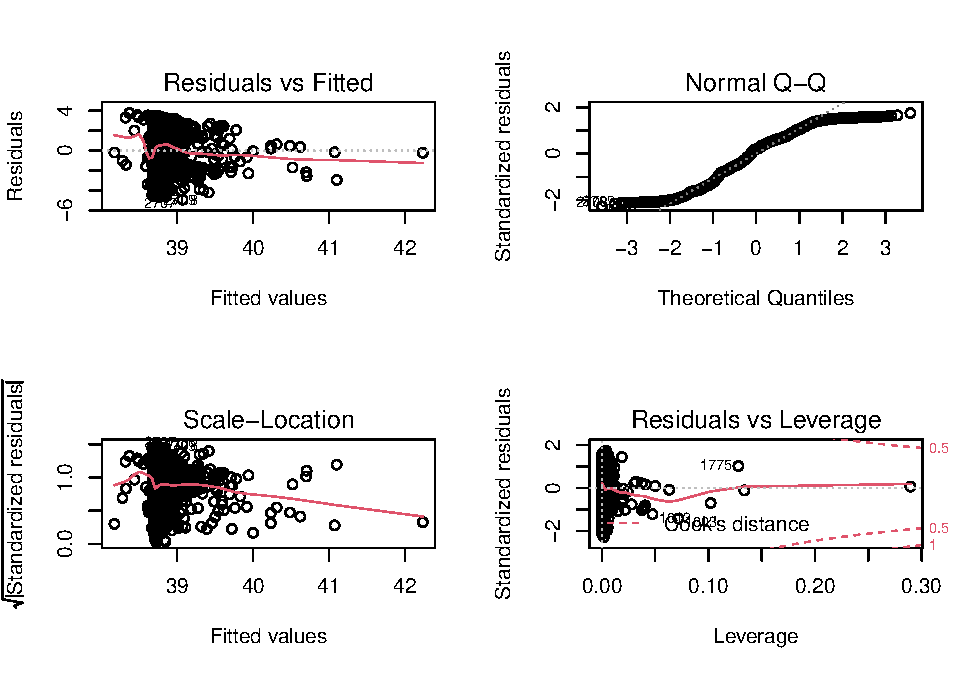
\includegraphics{Project_files/figure-latex/groundwater and river discharge-1.pdf}

\begin{Shaded}
\begin{Highlighting}[]
\FunctionTok{ggplot}\NormalTok{(data5, }\FunctionTok{aes}\NormalTok{(Groundwater\_Table\_feet))}\SpecialCharTok{+}
  \FunctionTok{theme}\NormalTok{(}\AttributeTok{text =} \FunctionTok{element\_text}\NormalTok{(}\AttributeTok{size =} \DecValTok{20}\NormalTok{))}\SpecialCharTok{+}
  \FunctionTok{geom\_point}\NormalTok{(}\FunctionTok{aes}\NormalTok{(}\AttributeTok{y=}\NormalTok{Flat\_Discharge, }\AttributeTok{color =} \StringTok{"Flat River"}\NormalTok{))}\SpecialCharTok{+}
    \FunctionTok{geom\_point}\NormalTok{(}\FunctionTok{aes}\NormalTok{(}\AttributeTok{y=}\NormalTok{Little\_Discharge, }\AttributeTok{color =} \StringTok{"Little River"}\NormalTok{))}\SpecialCharTok{+}
  \FunctionTok{xlab}\NormalTok{(}\StringTok{"Groundwater table/ft"}\NormalTok{)}\SpecialCharTok{+}\FunctionTok{ylab}\NormalTok{(}\StringTok{"River Discharge (sqft/s)"}\NormalTok{)}
\end{Highlighting}
\end{Shaded}

\begin{verbatim}
## Warning: Removed 2 rows containing missing values (geom_point).
\end{verbatim}

\begin{verbatim}
## Warning: Removed 5 rows containing missing values (geom_point).
\end{verbatim}

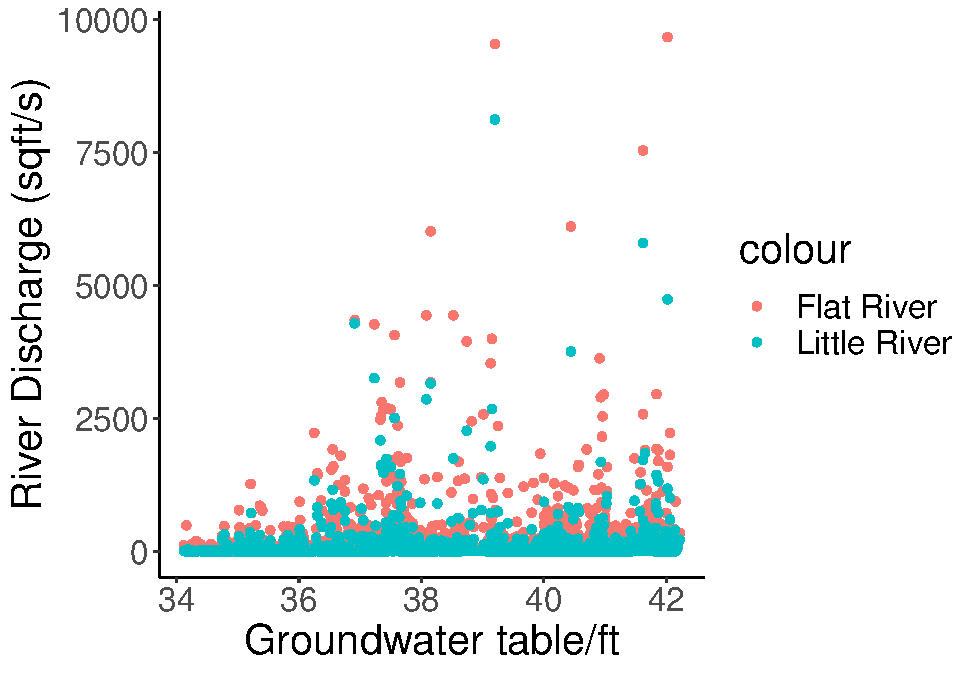
\includegraphics{Project_files/figure-latex/groundwater and river discharge-2.pdf}

\newpage

\hypertarget{summary-and-conclusions}{%
\section{Summary and Conclusions}\label{summary-and-conclusions}}

The results show that there is no significant correlation between the
municipal withdrawals and river discharge. At the same time, there is no
significant correlation between the precipitation and groundwater table
level. For Cape Fear River, there is a negative correlation with
precipitation. For Flat River, there are positive correlations with both
precipitation and groundwater table level. For Little River, there are
negative correlations with both precipitation and groundwater table
level. For the groundwater table level in Durham, there is a negative
correlation with municipal withdrawals. From the time-series analysis,
we conclude that the water capacity of the Durham region can remain
stable over a certain period of time and provide sufficient water for
regional development, human activities. And the analysis proves that the
effect of urban water use on river discharge is not significant. It is
the natural factors such as precipitation and groundwater table that
impact on the river discharge most.

In order to assess the stability of the North Carolina water market and
the scope for future development, we analyzed factors that may affect
the capacity of surface water resources, including precipitation, water
withdrawals. Through time-series analysis and regression analysis, we
concluded that the impact of municipal withdrawals on river discharge is
not significant, while precipitation and groundwater have a great impact
on river flow. The rivers around Durham can maintain a stable amount of
water for a certain period of time in the future. The current analysis
is deficient. One possible problem is that we could not obtain the
accurate groundwater capacity and groundwater use in North Carolina.
Recording changes in groundwater levels greatly reduces the magnitude of
changes in groundwater volume. The neglect of this variable may lead to
blind optimism about water resource capacity. Therefore, in the future,
the accurate data on groundwater is expected to be available to improve
this analysis. Another factor that biases the results is that although
we do not consider the effect of sewage volume as a factor on river flow
because the water withdrawal and discharge points for Durham are located
in different rivers, we cannot guarantee that other cities are not
discharging sewage to the studied rivers. Similarly, we cannot determine
whether the studied river is used as a water source only in Durham.
These could have some influence on the experimental results. Therefore,
in further studies, we need to identify all withdrawal and discharge
points in the studied rivers. In the more than 60 years since the
development of water resources management, the primary goal of water
resources development has been to support the economy and to identify
ways to increase freshwater supplies to meet anticipated demand (Gleick,
1998).With broadened consideration that includes issues of
sustainability and equity, a new debate on water policy has now begun,
as reflected by the statements coming from the 1992 Dublin statement,
Agenda 21 from Rio, the World Bank, and the Global Water Partnership.
The core arguments of the debate are that incorporating sustainability
and equity features into water resources planning and policy goals has
become a major policy priority, and this requires a high priority to
maintain the integrity of water resources and the flora and fauna and
human societies that develop around them. This argument is possible
because there is already a consensus that economic and environmental
constraints on resource development may shape future global groundwater
depletion. Not only the volume of physically available water needs to be
explored, but also the volume of water that is economically and
environmentally exploitable. Then understand how these limitations
affect the assessment of when aquifers become unsuitable for human
applications (Turner et al., 2019).

\newpage

\hypertarget{references}{%
\section{References}\label{references}}

A. E. Ercin, A. Y. Hoekstra, Water footprint scenarios for 2050: A
global analysis. Environ. Int. 64, 71-82 (2014). Boretti A., Rosa L.,
Reassessing the projections of the World Water Development Report. Clean
Water, 15 (2019). C. J. Vörösmarty, P. Green, J. Salisbury, R. B.
Lammers, Global water resources: Vulnerability from climate change and
population growth. Science. 289, 284-288 (2000). Brown T. C., Foti R.,
Ramirez J. A., Projected freshwater withdrawals in the United States
under a changing climate. Water Resources Research. 49, 1259--1276
(2013). Fan Y.B., Yang W. b., Li G., Wu L. L., Wei Y. S., Reuse rate of
treated wastewater in water reuse system. Journal of Environmental
Sciences. 17, 842-845, (2005). Gleick P. H., Water in crisis: paths to
sustainable water use. Ecological Applications. 8(3), 572-579 (1998).\\
M. M. Mekonnen, A. Y. Hoekstra, Four billion people facing severe water
scarcity. Sci Adv. 2 (2) (2016). Oki, T., and S. Kanae (2006), Global
hydrologic cycles and world water resources, Science, 313, 1068--1072.
R. G. Taylor, B. Scanlon, P. Döll, M. Rodell, R. van Beek, Y. Wada, L.
Longuevergne, M. Leblanc, J. S. Famiglietti, M. Edmunds, L. Konikow, T.
R. Green, J. Chen, M. Taniguchi, M. F. P. Bierkens, A. MacDonald, Y.
Fan, R. M. Maxwell, Y. Yechieli, J. J. Gurdak, D. M. Allen, M.
Shamsudduha, K. Hiscock, P. J.-F. Yeh, I. Holman, H. Treidel, Ground
water and climate change. Nat. Clim. Chang. 3, 322--329 (2013). S.
Siebert, J. Burke, J. M. Faures, K. Frenken, J. Hoogeveen, P. Döll, F.
T. Portmann, Groundwater use for irrigation -- a global inventory.
Hydrol. Earth Syst. Sci. 14, 1863--1880 (2010). Turner, S. W. D.,
Hejazi, M., Yonkofski, C., Kim, S. H., \& Page, K., Influence of
groundwater extraction costs and resource depletion limits on simulated
global nonrenewable water withdrawals over the Twenty‐First century.
Earth's Future, 7(2), 123-135 (2019). World Water Assessment Programme
(Nations Unies), The United Nations World Water Development Report 2018
(United Nations Educational, Scientific and Cultural Organization, New
York, United States)
www.unwater.org/publications/world-water-development-report-2018/.
(2018). Y. Wada, L. P. H. van Beek, D. Viviroli, H. H. Dürr, R.
Weingartner, M. F. P. Bierkens, Global monthly water stress: 2. Water
demand and severity of water stress. Water Resour. Res. 47, W07518
(2011).

\end{document}
